% Options for packages loaded elsewhere
\PassOptionsToPackage{unicode}{hyperref}
\PassOptionsToPackage{hyphens}{url}
\PassOptionsToPackage{dvipsnames,svgnames,x11names}{xcolor}
%
\documentclass[
  letterpaper,
  DIV=11,
  numbers=noendperiod]{scrreport}

\usepackage{amsmath,amssymb}
\usepackage{lmodern}
\usepackage{iftex}
\ifPDFTeX
  \usepackage[T1]{fontenc}
  \usepackage[utf8]{inputenc}
  \usepackage{textcomp} % provide euro and other symbols
\else % if luatex or xetex
  \usepackage{unicode-math}
  \defaultfontfeatures{Scale=MatchLowercase}
  \defaultfontfeatures[\rmfamily]{Ligatures=TeX,Scale=1}
\fi
% Use upquote if available, for straight quotes in verbatim environments
\IfFileExists{upquote.sty}{\usepackage{upquote}}{}
\IfFileExists{microtype.sty}{% use microtype if available
  \usepackage[]{microtype}
  \UseMicrotypeSet[protrusion]{basicmath} % disable protrusion for tt fonts
}{}
\makeatletter
\@ifundefined{KOMAClassName}{% if non-KOMA class
  \IfFileExists{parskip.sty}{%
    \usepackage{parskip}
  }{% else
    \setlength{\parindent}{0pt}
    \setlength{\parskip}{6pt plus 2pt minus 1pt}}
}{% if KOMA class
  \KOMAoptions{parskip=half}}
\makeatother
\usepackage{xcolor}
\setlength{\emergencystretch}{3em} % prevent overfull lines
\setcounter{secnumdepth}{5}
% Make \paragraph and \subparagraph free-standing
\ifx\paragraph\undefined\else
  \let\oldparagraph\paragraph
  \renewcommand{\paragraph}[1]{\oldparagraph{#1}\mbox{}}
\fi
\ifx\subparagraph\undefined\else
  \let\oldsubparagraph\subparagraph
  \renewcommand{\subparagraph}[1]{\oldsubparagraph{#1}\mbox{}}
\fi

\usepackage{color}
\usepackage{fancyvrb}
\newcommand{\VerbBar}{|}
\newcommand{\VERB}{\Verb[commandchars=\\\{\}]}
\DefineVerbatimEnvironment{Highlighting}{Verbatim}{commandchars=\\\{\}}
% Add ',fontsize=\small' for more characters per line
\usepackage{framed}
\definecolor{shadecolor}{RGB}{241,243,245}
\newenvironment{Shaded}{\begin{snugshade}}{\end{snugshade}}
\newcommand{\AlertTok}[1]{\textcolor[rgb]{0.68,0.00,0.00}{#1}}
\newcommand{\AnnotationTok}[1]{\textcolor[rgb]{0.37,0.37,0.37}{#1}}
\newcommand{\AttributeTok}[1]{\textcolor[rgb]{0.40,0.45,0.13}{#1}}
\newcommand{\BaseNTok}[1]{\textcolor[rgb]{0.68,0.00,0.00}{#1}}
\newcommand{\BuiltInTok}[1]{\textcolor[rgb]{0.00,0.23,0.31}{#1}}
\newcommand{\CharTok}[1]{\textcolor[rgb]{0.13,0.47,0.30}{#1}}
\newcommand{\CommentTok}[1]{\textcolor[rgb]{0.37,0.37,0.37}{#1}}
\newcommand{\CommentVarTok}[1]{\textcolor[rgb]{0.37,0.37,0.37}{\textit{#1}}}
\newcommand{\ConstantTok}[1]{\textcolor[rgb]{0.56,0.35,0.01}{#1}}
\newcommand{\ControlFlowTok}[1]{\textcolor[rgb]{0.00,0.23,0.31}{#1}}
\newcommand{\DataTypeTok}[1]{\textcolor[rgb]{0.68,0.00,0.00}{#1}}
\newcommand{\DecValTok}[1]{\textcolor[rgb]{0.68,0.00,0.00}{#1}}
\newcommand{\DocumentationTok}[1]{\textcolor[rgb]{0.37,0.37,0.37}{\textit{#1}}}
\newcommand{\ErrorTok}[1]{\textcolor[rgb]{0.68,0.00,0.00}{#1}}
\newcommand{\ExtensionTok}[1]{\textcolor[rgb]{0.00,0.23,0.31}{#1}}
\newcommand{\FloatTok}[1]{\textcolor[rgb]{0.68,0.00,0.00}{#1}}
\newcommand{\FunctionTok}[1]{\textcolor[rgb]{0.28,0.35,0.67}{#1}}
\newcommand{\ImportTok}[1]{\textcolor[rgb]{0.00,0.46,0.62}{#1}}
\newcommand{\InformationTok}[1]{\textcolor[rgb]{0.37,0.37,0.37}{#1}}
\newcommand{\KeywordTok}[1]{\textcolor[rgb]{0.00,0.23,0.31}{#1}}
\newcommand{\NormalTok}[1]{\textcolor[rgb]{0.00,0.23,0.31}{#1}}
\newcommand{\OperatorTok}[1]{\textcolor[rgb]{0.37,0.37,0.37}{#1}}
\newcommand{\OtherTok}[1]{\textcolor[rgb]{0.00,0.23,0.31}{#1}}
\newcommand{\PreprocessorTok}[1]{\textcolor[rgb]{0.68,0.00,0.00}{#1}}
\newcommand{\RegionMarkerTok}[1]{\textcolor[rgb]{0.00,0.23,0.31}{#1}}
\newcommand{\SpecialCharTok}[1]{\textcolor[rgb]{0.37,0.37,0.37}{#1}}
\newcommand{\SpecialStringTok}[1]{\textcolor[rgb]{0.13,0.47,0.30}{#1}}
\newcommand{\StringTok}[1]{\textcolor[rgb]{0.13,0.47,0.30}{#1}}
\newcommand{\VariableTok}[1]{\textcolor[rgb]{0.07,0.07,0.07}{#1}}
\newcommand{\VerbatimStringTok}[1]{\textcolor[rgb]{0.13,0.47,0.30}{#1}}
\newcommand{\WarningTok}[1]{\textcolor[rgb]{0.37,0.37,0.37}{\textit{#1}}}

\providecommand{\tightlist}{%
  \setlength{\itemsep}{0pt}\setlength{\parskip}{0pt}}\usepackage{longtable,booktabs,array}
\usepackage{calc} % for calculating minipage widths
% Correct order of tables after \paragraph or \subparagraph
\usepackage{etoolbox}
\makeatletter
\patchcmd\longtable{\par}{\if@noskipsec\mbox{}\fi\par}{}{}
\makeatother
% Allow footnotes in longtable head/foot
\IfFileExists{footnotehyper.sty}{\usepackage{footnotehyper}}{\usepackage{footnote}}
\makesavenoteenv{longtable}
\usepackage{graphicx}
\makeatletter
\def\maxwidth{\ifdim\Gin@nat@width>\linewidth\linewidth\else\Gin@nat@width\fi}
\def\maxheight{\ifdim\Gin@nat@height>\textheight\textheight\else\Gin@nat@height\fi}
\makeatother
% Scale images if necessary, so that they will not overflow the page
% margins by default, and it is still possible to overwrite the defaults
% using explicit options in \includegraphics[width, height, ...]{}
\setkeys{Gin}{width=\maxwidth,height=\maxheight,keepaspectratio}
% Set default figure placement to htbp
\makeatletter
\def\fps@figure{htbp}
\makeatother

\KOMAoption{captions}{tableheading}
\makeatletter
\@ifpackageloaded{tcolorbox}{}{\usepackage[many]{tcolorbox}}
\@ifpackageloaded{fontawesome5}{}{\usepackage{fontawesome5}}
\definecolor{quarto-callout-color}{HTML}{909090}
\definecolor{quarto-callout-note-color}{HTML}{0758E5}
\definecolor{quarto-callout-important-color}{HTML}{CC1914}
\definecolor{quarto-callout-warning-color}{HTML}{EB9113}
\definecolor{quarto-callout-tip-color}{HTML}{00A047}
\definecolor{quarto-callout-caution-color}{HTML}{FC5300}
\definecolor{quarto-callout-color-frame}{HTML}{acacac}
\definecolor{quarto-callout-note-color-frame}{HTML}{4582ec}
\definecolor{quarto-callout-important-color-frame}{HTML}{d9534f}
\definecolor{quarto-callout-warning-color-frame}{HTML}{f0ad4e}
\definecolor{quarto-callout-tip-color-frame}{HTML}{02b875}
\definecolor{quarto-callout-caution-color-frame}{HTML}{fd7e14}
\makeatother
\makeatletter
\makeatother
\makeatletter
\@ifpackageloaded{bookmark}{}{\usepackage{bookmark}}
\makeatother
\makeatletter
\@ifpackageloaded{caption}{}{\usepackage{caption}}
\AtBeginDocument{%
\ifdefined\contentsname
  \renewcommand*\contentsname{Indice de contenidos}
\else
  \newcommand\contentsname{Indice de contenidos}
\fi
\ifdefined\listfigurename
  \renewcommand*\listfigurename{Listado de Figuras}
\else
  \newcommand\listfigurename{Listado de Figuras}
\fi
\ifdefined\listtablename
  \renewcommand*\listtablename{Listado de Tablas}
\else
  \newcommand\listtablename{Listado de Tablas}
\fi
\ifdefined\figurename
  \renewcommand*\figurename{Figura}
\else
  \newcommand\figurename{Figura}
\fi
\ifdefined\tablename
  \renewcommand*\tablename{Tabla}
\else
  \newcommand\tablename{Tabla}
\fi
}
\@ifpackageloaded{float}{}{\usepackage{float}}
\floatstyle{ruled}
\@ifundefined{c@chapter}{\newfloat{codelisting}{h}{lop}}{\newfloat{codelisting}{h}{lop}[chapter]}
\floatname{codelisting}{Listado}
\newcommand*\listoflistings{\listof{codelisting}{Listado de Listatdos}}
\makeatother
\makeatletter
\@ifpackageloaded{caption}{}{\usepackage{caption}}
\@ifpackageloaded{subcaption}{}{\usepackage{subcaption}}
\makeatother
\makeatletter
\@ifpackageloaded{tcolorbox}{}{\usepackage[many]{tcolorbox}}
\makeatother
\makeatletter
\@ifundefined{shadecolor}{\definecolor{shadecolor}{rgb}{.97, .97, .97}}
\makeatother
\makeatletter
\makeatother
\ifLuaTeX
\usepackage[bidi=basic]{babel}
\else
\usepackage[bidi=default]{babel}
\fi
\babelprovide[main,import]{spanish}
% get rid of language-specific shorthands (see #6817):
\let\LanguageShortHands\languageshorthands
\def\languageshorthands#1{}
\ifLuaTeX
  \usepackage{selnolig}  % disable illegal ligatures
\fi
\IfFileExists{bookmark.sty}{\usepackage{bookmark}}{\usepackage{hyperref}}
\IfFileExists{xurl.sty}{\usepackage{xurl}}{} % add URL line breaks if available
\urlstyle{same} % disable monospaced font for URLs
\hypersetup{
  pdftitle={Manual de LaTeX},
  pdfauthor={Alfredo Sánchez Alberca},
  pdflang={es},
  colorlinks=true,
  linkcolor={blue},
  filecolor={Maroon},
  citecolor={Blue},
  urlcolor={Blue},
  pdfcreator={LaTeX via pandoc}}

\title{Manual de LaTeX}
\author{Alfredo Sánchez Alberca}
\date{6/1/2022}

\begin{document}
\maketitle
\ifdefined\Shaded\renewenvironment{Shaded}{\begin{tcolorbox}[breakable, interior hidden, frame hidden, boxrule=0pt, borderline west={3pt}{0pt}{shadecolor}, enhanced, sharp corners]}{\end{tcolorbox}}\fi

\renewcommand*\contentsname{Indice de contenidos}
{
\hypersetup{linkcolor=}
\setcounter{tocdepth}{2}
\tableofcontents
}
\bookmarksetup{startatroot}

\hypertarget{prefacio}{%
\chapter*{Prefacio}\label{prefacio}}
\addcontentsline{toc}{chapter}{Prefacio}

¡Bienvenida/os al manual de \LaTeX.!

Este libro presenta una introducción al lenguaje de composición de
textos \href{https://www.latex-project.org/}{\LaTeX} con un enfoque
orientado a la creación de documentos científicos y técnicos con
contenido matemático.

\hypertarget{licencia}{%
\section*{Licencia}\label{licencia}}
\addcontentsline{toc}{section}{Licencia}

Esta obra está bajo una licencia Reconocimiento -- No comercial --
Compartir bajo la misma licencia 3.0 España de Creative Commons. Para
ver una copia de esta licencia, visite
\url{https://creativecommons.org/licenses/by-nc-sa/3.0/es/}.

Con esta licencia eres libre de:

\begin{itemize}
\tightlist
\item
  Copiar, distribuir y mostrar este trabajo.
\item
  Realizar modificaciones de este trabajo.
\end{itemize}

Bajo las siguientes condiciones:

\begin{itemize}
\item
  \textbf{Reconocimiento}. Debe reconocer los créditos de la obra de la
  manera especificada por el autor o el licenciador (pero no de una
  manera que sugiera que tiene su apoyo o apoyan el uso que hace de su
  obra).
\item
  \textbf{No comercial}. No puede utilizar esta obra para fines
  comerciales.
\item
  \textbf{Compartir bajo la misma licencia}. Si altera o transforma esta
  obra, o genera una obra derivada, sólo puede distribuir la obra
  generada bajo una licencia idéntica a ésta.
\end{itemize}

Al reutilizar o distribuir la obra, tiene que dejar bien claro los
términos de la licencia de esta obra.

Estas condiciones pueden no aplicarse si se obtiene el permiso del
titular de los derechos de autor.

Nada en esta licencia menoscaba o restringe los derechos morales del
autor.

\bookmarksetup{startatroot}

\hypertarget{introducciuxf3n}{%
\chapter{Introducción}\label{introducciuxf3n}}

\hypertarget{quuxe9-es-tex}{%
\section{\texorpdfstring{¿Qué es
\TeX?}{¿Qué es \textbackslash TeX?}}\label{quuxe9-es-tex}}

\TeX es un sistema de composición de documentos de alta calidad,
orientado especialmente a la creación de documentos científicos y
técnicos que incluyen fórmulas matemáticas. Fue creado por
\href{https://es.wikipedia.org/wiki/Donald_Knuth}{Donald Knuth} en 1978.

A diferencia de un procesador de textos como por ejemplo Microsoft Word,
\TeX no es una aplicación sino un lenguaje de programación que
require compilar el código fuente para obtener el documento final. Esto,
que a priori podría parecer una desventaja, en realidad es la gran
ventaja de \TeX frente a los procesadores de texto que siguen el
paradigma \href{https://es.wikipedia.org/wiki/WYSIWYG}{WYSIWYG}
(\emph{What You See Is What You Get}), ya que permite separar fácilmente
el contenido y la estructura de un documento, de su formato, de manera
que el usuario puede centrarse en el contenido y la estructura del
documento, y dejar que \TeX se encargue del formato. De hecho,
\TeX incorpora un potente
\href{https://es.wikipedia.org/wiki/Lenguaje_de_marcado}{lenguaje de
marcado} para estructurar y formatear el texto de un documento. Por
ejemplo, mientras que para poner una palabra en negrita con un
procesador de textos como Microsoft Word, bastaría con seleccionar la
palabra y hacer clic en el botón de negrita para ver automáticamente la
palabra en negrita en la pantalla del ordenador, en \TeX habría que
escribir en el fichero con el código fuente
\texttt{\{\textbackslash{}bf\ palabra\}} y después compilar el código
fuente para obtener un documento final con la palabra en negrita (el
comando \texttt{\textbackslash{}bf}, que permite aplicar la negrita, se
conoce como \emph{marca} o \emph{tag} en inglés.)

La página principal con información sobre \TeX es la del
\href{https://www.tug.org/}{TeX Users Group}.

\hypertarget{quuxe9-es-latex}{%
\section{\texorpdfstring{¿Qué es
\LaTeX}{¿Qué es \textbackslash LaTeX}}\label{quuxe9-es-latex}}


\includegraphics{./img/logos/latex-project-logo.png}

\LaTeX es un conjunto de macros para \TeX debido originalmente a
\href{https://en.wikipedia.org/wiki/Leslie_Lamport}{Leslie Lamport} para
facilitar el uso de \TeX.

Tanto \TeX como \LaTeX son programas de código abierto,
liberados bajo la \href{https://www.latex-project.org/lppl.txt}{licencia
LPPL}.

Otra de las grandes ventajas de \LaTeX es que existen multitud de
paquetes de código libre para generar distintos tipos de documentos que
pueden descargarse desde el repositorio \href{https://ctan.org/}{CRAN}.

La página principal sobre \LaTeX es
\href{https://www.latex-project.org/}{The LaTeX project}.

\hypertarget{instalaciuxf3n}{%
\section{Instalación}\label{instalaciuxf3n}}

Existen distintas distribuciones de \LaTeX y algunas de ellas son
multiplataforma, es decir, están disponibles para diferentes sistemas
operativos. Las distribuciones más comunes son:

\begin{itemize}
\tightlist
\item
  \href{https://tug.org/texlive/}{TeXLive} para Windows, Mac OSX y
  Linux.
\item
  \href{}{MiKTeX} para Windows, Mac OSX y Linux.
\item
  \href{https://www.tug.org/mactex/}{MacTeX} para Mac OSX.
\end{itemize}

En sus respectivas páginas está explicado el procedimiento de
instalación de cada una.

Junto a la distribución de \LaTeX es también habitual instalar algún
editor de texto para escribir el código fuente. En realidad puede usarse
cualquier editor de texto que ya esté instalado en nuestro sistema
operativo, pero los existen entornos de edición especializados que
facilitan muchas de las tareas del proceso de composición de documentos
con \LaTeX. Los más comunes son:

\begin{itemize}
\tightlist
\item
  \href{http://www.xm1math.net/texmaker/}{TexMaker}. Es un editor de
  texto libre, multiplataforma, con muchos asistentes disponibles que
  permite previsualizar en tiempo real el documento final en pdf
\item
  \href{http://www.texstudio.org/}{Texstudio}. Es otro editor libre y
  multiplataforma que incorpora aún más asistentes que el anterior.
\item
  \href{https://www.vim.org/}{Vim} Es un editor de texto simple de
  propósito general que también es libre y multiplataforma. Incorpora
  paquetes o plugins específicos para facilitar la creación de
  documentos con \LaTeX. Especialmente indicado para trabajar desde
  la terminal.
\item
  \href{https://www.gnu.org/software/emacs/}{Emacs}. Es otro editor
  similar a Vim, muy extendido entre los usuarios que prefieren usar la
  terminal.
\item
  \href{https://code.visualstudio.com/}{Visual Studio Code}. Es un
  potente entorno de desarrollo multipropósito. Dispone de paquetes para
  los lenguajes de programación más comunes, entre ellos \LaTeX.
\end{itemize}

Pero también se puede empezar a componer documentos sin necesidad de
instalar nada en el ordenador, usando un editor on-line como por ejemplo
\href{https://www.overleaf.com/}{Overleaf}

\hypertarget{hola-latex}{%
\section{Hola LaTeX}\label{hola-latex}}

A modo de ejemplo, empezaremos por crear un sencillo documento con el
texto ``Hola \LaTeX''.

Para ello utilizaremos nuestro editor de texto preferido para crear un
fichero de texto con el nombre \texttt{main.tex} y el siguiente
contenido:

\begin{Shaded}
\begin{Highlighting}[]
\BuiltInTok{\textbackslash{}documentclass}\NormalTok{\{}\ExtensionTok{article}\NormalTok{\}}
\KeywordTok{\textbackslash{}begin}\NormalTok{\{}\ExtensionTok{document}\NormalTok{\}}
\NormalTok{Hola }\FunctionTok{\textbackslash{}LaTeX}
\KeywordTok{\textbackslash{}end}\NormalTok{\{}\ExtensionTok{document}\NormalTok{\}}
\end{Highlighting}
\end{Shaded}

\begin{tcolorbox}[enhanced jigsaw, arc=.35mm, toprule=.15mm, opacitybacktitle=0.6, colback=white, coltitle=black, colbacktitle=quarto-callout-important-color!10!white, breakable, colframe=quarto-callout-important-color-frame, left=2mm, opacityback=0, bottomtitle=1mm, toptitle=1mm, titlerule=0mm, title=\textcolor{quarto-callout-important-color}{\faExclamation}\hspace{0.5em}{Importante}, bottomrule=.15mm, leftrule=.75mm, rightrule=.15mm]
El nombre del fichero de texto con el código fuente de \LaTeX puede
ser el que queramos, pero es importante que la extensión sea
\texttt{.tex},
\end{tcolorbox}

Aunque más adelante se verá la estructura general del código fuente de
un documento en \LaTeX, a continuación se explica brevemente el
contenido de este fichero:

\begin{enumerate}
\def\labelenumi{\arabic{enumi}.}
\tightlist
\item
  En la primera línea se especifica el tipo de documento
  (\texttt{article}).
\item
  En la segunda línea se especifica el idioma del documento
  (\texttt{spanish}).
\item
  La tercera línea marca el comienzo del documento.
\item
  La cuarta línea contiene el texto del documento.
  \texttt{\textbackslash{}LaTeX} es un comando que produce la salida
  \LaTeX.
\item
  La quinta línea marca el final del documento.
\end{enumerate}

\hypertarget{compilaciuxf3n}{%
\subsection{Compilación}\label{compilaciuxf3n}}

Para obtener el documento final hay que compilar el fichero fuente.
Existen diferentes formas de hacerlo y en los editores anteriores suele
ser tan sencillo como hacer clic en un botón o pulsar una combinación de
teclas, pero en última instancia todos ellos hacen una llamada al
compilador de \LaTeX que es quien se encarga de convertir el código
fuente en el documento final.

Cada distribución de \LaTeX viene con varios compiladores. Los más
habituales son:

\begin{itemize}
\tightlist
\item
  \texttt{latex}: Es el compilador más antiguo y genera documentos en
  \href{https://es.wikipedia.org/wiki/DVI_(TeX)}{formato \texttt{dvi}},
  que es un formato independiente creado mucho antes que el formato
  \texttt{pdf}.
\item
  \href{https://www.tug.org/applications/pdftex/}{\texttt{pdflatex}}: Es
  el compilador más usado y genera documentos en formato \texttt{pdf}.
\item
  \href{https://tug.org/xetex/}{\texttt{xelatex}}: Es un compilador más
  moderno que admite caracteres Unicode en el código fuente y el uso de
  tipografías más modernas.
\end{itemize}

En una terminal, la compilación de este documento sería tecleando el
comando \texttt{latex\ main.tex}, \texttt{pdflatex\ main.tex} o
\texttt{xelatex\ main.tex}, dependiendo del compilador que se quiera
usar. A continuación se muestra la salida que general el compilador
\texttt{pdflatex} al compilar el fichero \texttt{main.tex}.

\begin{Shaded}
\begin{Highlighting}[]
\OperatorTok{\textgreater{}}\NormalTok{ pdflatex }\ExtensionTok{main.tex} 
\ExtensionTok{s}\NormalTok{ is pdfTeX, Version 3.141592653{-}2.6{-}1.40.22 }\ErrorTok{(}\ExtensionTok{TeX}\NormalTok{ Live 2021}\KeywordTok{)} \KeywordTok{(}\ExtensionTok{preloaded} 
\VariableTok{format}\OperatorTok{=}\NormalTok{pdflatex}\KeywordTok{)} \ExtensionTok{restricted} \DataTypeTok{\textbackslash{}w}\NormalTok{rite18 enabled.}
\ExtensionTok{entering}\NormalTok{ extended mode}
\KeywordTok{(}\ExtensionTok{./main.tex}
\ExtensionTok{LaTeX2e} \OperatorTok{\textless{}}\NormalTok{2021{-}06{-}01}\OperatorTok{\textgreater{}}\NormalTok{ patch level 1}
\ExtensionTok{L3}\NormalTok{ programming layer }\OperatorTok{\textless{}}\NormalTok{2021{-}06{-}18}\OperatorTok{\textgreater{}}
\KeywordTok{(}\ExtensionTok{/usr/local/texlive/2021/texmf{-}dist/tex/latex/base/article.cls}
\ExtensionTok{Document}\NormalTok{ Class: article 2021/02/12 v1.4n Standard LaTeX document class}
\KeywordTok{(}\ExtensionTok{/usr/local/texlive/2021/texmf{-}dist/tex/latex/base/size10.clo}\KeywordTok{))}
\KeywordTok{(}\ExtensionTok{/usr/local/texlive/2021/texmf{-}dist/tex/generic/babel/babel.sty}
\KeywordTok{(}\ExtensionTok{/usr/local/texlive/2021/texmf{-}dist/tex/generic/babel/babel.def}
\KeywordTok{(}\ExtensionTok{/usr/local/texlive/2021/texmf{-}dist/tex/generic/babel/txtbabel.def}\KeywordTok{))}
\KeywordTok{(}\ExtensionTok{/usr/local/texlive/2021/texmf{-}dist/tex/generic/babel{-}spanish/spanish.ldf}\KeywordTok{))}
\KeywordTok{(}\ExtensionTok{/usr/local/texlive/2021/texmf{-}dist/tex/latex/l3backend/l3backend{-}pdftex.def}\KeywordTok{)}
\KeywordTok{(}\ExtensionTok{./main.aux}\KeywordTok{)} \ExtensionTok{[1\{/usr/local/texlive/2021/texmf{-}var/fonts/map/pdftex/updmap/}
\ExtensionTok{pdftex.map\}]} \ErrorTok{(}\ExtensionTok{./main.aux}\KeywordTok{)} \KeywordTok{)}\OperatorTok{\textless{}}\NormalTok{/usr/local/texlive/2021/texmf{-}dist/fonts/type1/}
\ExtensionTok{public/amsfonts/cm/cmr10.pfb}\OperatorTok{\textgreater{}\textless{}}\NormalTok{/usr/local/texlive/2021/texmf{-}dist/fonts/type1/}
\ExtensionTok{public/amsfonts/cm/cmr7.pfb}\OperatorTok{\textgreater{}}
\ExtensionTok{Output}\NormalTok{ written on main.pdf }\ErrorTok{(}\ExtensionTok{1}\NormalTok{ page, 20106 bytes}\KeywordTok{)}\BuiltInTok{.}
\ExtensionTok{Transcript}\NormalTok{ written on main.log.}
\end{Highlighting}
\end{Shaded}

En la Figura~\ref{fig-overleaf-hola-latex} se puede apreciar el
documento final que se obtiene tras compilar el código fuente en
Overleaf.

\begin{figure}

{\centering 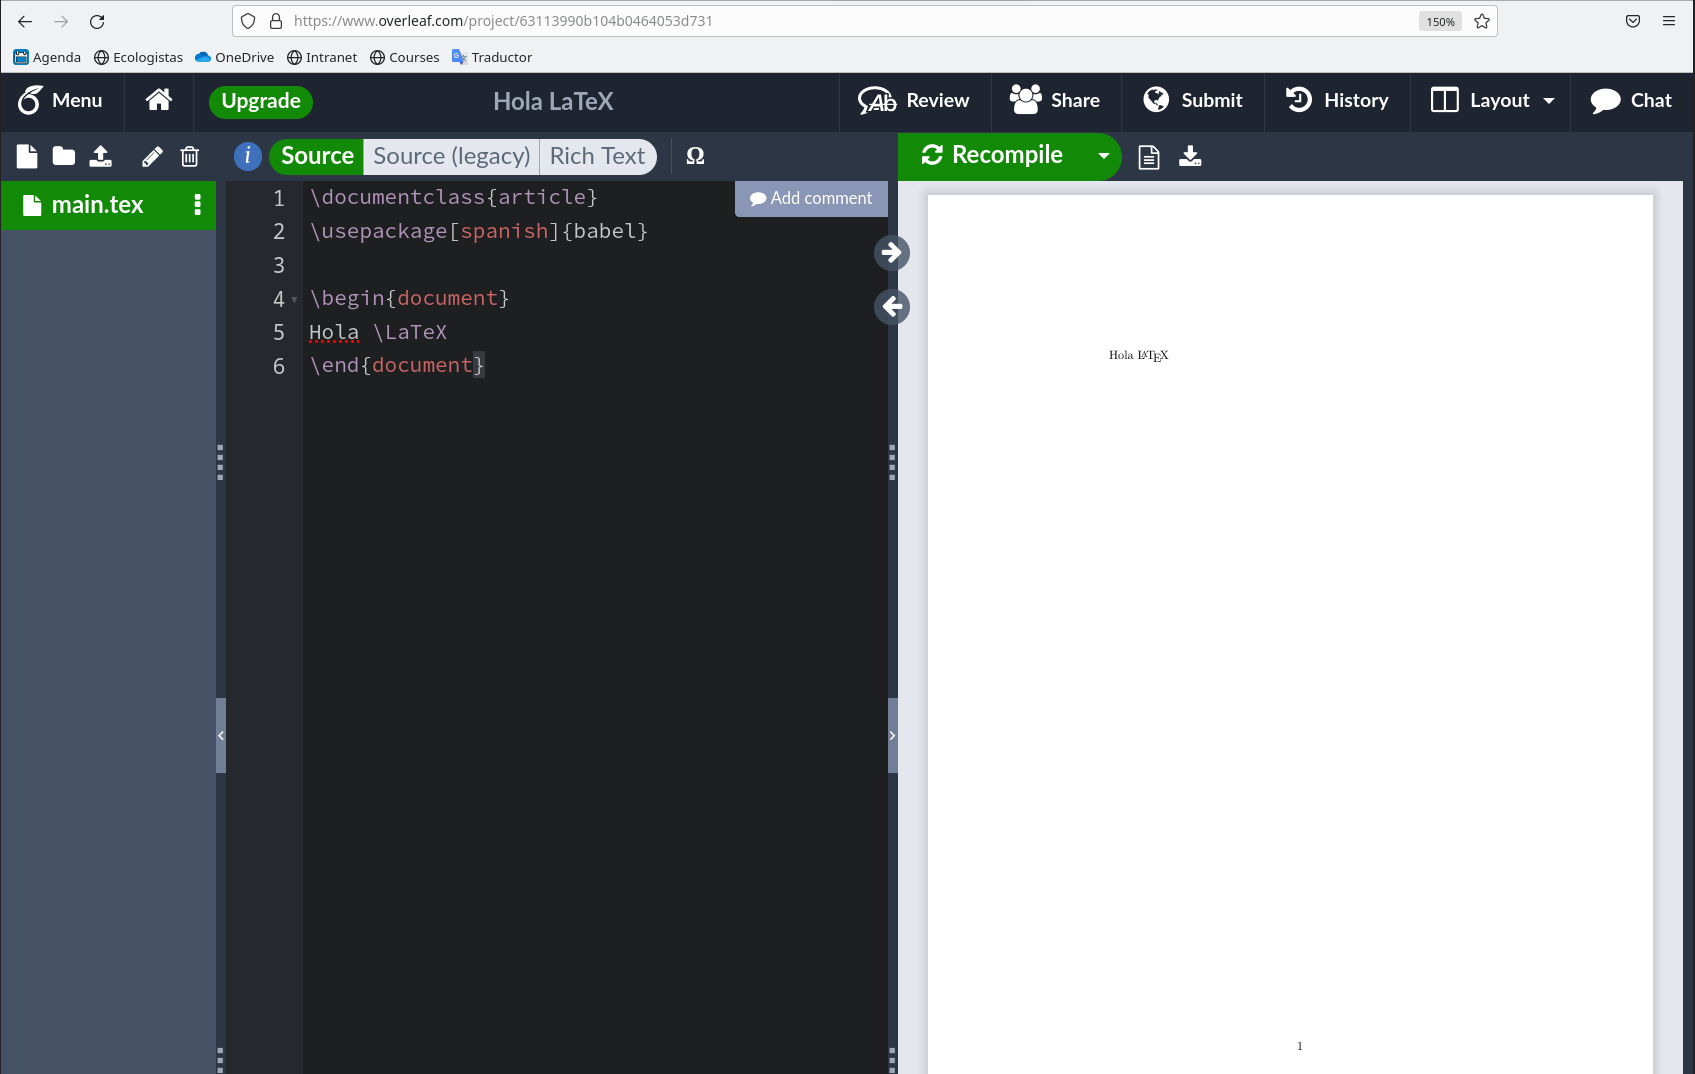
\includegraphics{./img/introduccion/overleaf-hola-latex.png}

}

\caption{\label{fig-overleaf-hola-latex}Creación de un documento en
Overleaf.}

\end{figure}

Al principio es muy habitual cometer errores en el código fuente, por lo
que el proceso de compilación fallará. En ese caso es importante leer
los mensajes de salida del compilador donde informará sobre el tipo de
error y la línea donde se produjo el error, lo que facilitará su
corrección. Algunos entornos de edición como por ejemplo Overleaf son
capaces de anticiparse a los errores de compilación y detectan errores
de sintaxis o gramaticales indicando el lugar exacto del error.

\textbf{Ejemplo}

Si en el documento anterior cambiamos el comando
\texttt{\textbackslash{}LaTeX} por otro que no existe, por ejemplo
\texttt{\textbackslash{}error}, al compilar el documento tendremos el
siguiente error.

\begin{Shaded}
\begin{Highlighting}[]
\OperatorTok{\textgreater{}}\NormalTok{ pdflatex }\ExtensionTok{main.tex}
\ExtensionTok{This}\NormalTok{ is pdfTeX, Version 3.141592653{-}2.6{-}1.40.22 }\ErrorTok{(}\ExtensionTok{TeX}\NormalTok{ Live 2021}\KeywordTok{)} \KeywordTok{(}\ExtensionTok{preloaded} 
\VariableTok{format}\OperatorTok{=}\NormalTok{pdflatex}\KeywordTok{)} \ExtensionTok{restricted} \DataTypeTok{\textbackslash{}w}\NormalTok{rite18 enabled.}
\ExtensionTok{entering}\NormalTok{ extended mode}
\KeywordTok{(}\ExtensionTok{./main.tex}
\ExtensionTok{LaTeX2e} \OperatorTok{\textless{}}\NormalTok{2021{-}06{-}01}\OperatorTok{\textgreater{}}\NormalTok{ patch level 1}
\ExtensionTok{L3}\NormalTok{ programming layer }\OperatorTok{\textless{}}\NormalTok{2021{-}06{-}18}\OperatorTok{\textgreater{}}
\KeywordTok{(}\ExtensionTok{/usr/local/texlive/2021/texmf{-}dist/tex/latex/base/article.cls}
\ExtensionTok{Document}\NormalTok{ Class: article 2021/02/12 v1.4n Standard LaTeX document class}
\KeywordTok{(}\ExtensionTok{/usr/local/texlive/2021/texmf{-}dist/tex/latex/base/size10.clo}\KeywordTok{))}
\KeywordTok{(}\ExtensionTok{/usr/local/texlive/2021/texmf{-}dist/tex/latex/l3backend/l3backend{-}pdftex.def}\KeywordTok{)}
\KeywordTok{(}\ExtensionTok{./main.aux}\KeywordTok{)}
\OtherTok{! }\ExtensionTok{Undefined}\NormalTok{ control sequence.}
\ExtensionTok{l.6}\NormalTok{ Ejemplo de documento con un error. }\DataTypeTok{\textbackslash{}e}\NormalTok{rror}
                                             
\ExtensionTok{?} 
\end{Highlighting}
\end{Shaded}

\begin{tcolorbox}[enhanced jigsaw, arc=.35mm, toprule=.15mm, opacitybacktitle=0.6, colback=white, coltitle=black, colbacktitle=quarto-callout-warning-color!10!white, breakable, colframe=quarto-callout-warning-color-frame, left=2mm, opacityback=0, bottomtitle=1mm, toptitle=1mm, titlerule=0mm, title=\textcolor{quarto-callout-warning-color}{\faExclamationTriangle}\hspace{0.5em}{Advertencia}, bottomrule=.15mm, leftrule=.75mm, rightrule=.15mm]
Si el documento contiene referencias cruzadas, citaciones
bibliográficas, tabla de contenidos o índices, es necesario compilar el
documento dos o tres veces para que se generen automáticamente esas
partes.
\end{tcolorbox}

\bookmarksetup{startatroot}

\hypertarget{estructura-de-un-documento}{%
\chapter{Estructura de un documento}\label{estructura-de-un-documento}}

\hypertarget{esqueleto-buxe1sico-para-pdflatex}{%
\section{\texorpdfstring{Esqueleto básico para
\texttt{pdflatex}}{Esqueleto básico para pdflatex}}\label{esqueleto-buxe1sico-para-pdflatex}}

El esqueleto básico del código fuente de un documento en español para
compilar con \texttt{latex} o \texttt{pdflatex} es el siguiente:

\begin{Shaded}
\begin{Highlighting}[]
\CommentTok{\% CLASE}
\BuiltInTok{\textbackslash{}documentclass}\NormalTok{[a4paper,10pt]\{}\ExtensionTok{article}\NormalTok{\}}

\CommentTok{\% PREÁMBULO}
\CommentTok{\% Paquetes}
\BuiltInTok{\textbackslash{}usepackage}\NormalTok{[utf8]\{}\ExtensionTok{inputenc}\NormalTok{\}}
\BuiltInTok{\textbackslash{}usepackage}\NormalTok{[spanish]\{}\ExtensionTok{babel}\NormalTok{\}}
\BuiltInTok{\textbackslash{}usepackage}\NormalTok{[T1]\{}\ExtensionTok{fontenc}\NormalTok{\}}

\CommentTok{\% Título, autor y fecha}
\FunctionTok{\textbackslash{}title}\NormalTok{\{Título\}}
\FunctionTok{\textbackslash{}author}\NormalTok{\{Autor\}}
\FunctionTok{\textbackslash{}date}\NormalTok{\{Fecha\}}

\CommentTok{\% CUERPO}
\KeywordTok{\textbackslash{}begin}\NormalTok{\{}\ExtensionTok{document}\NormalTok{\}}

\FunctionTok{\textbackslash{}maketitle}

\CommentTok{\% Resumen}
\KeywordTok{\textbackslash{}begin}\NormalTok{\{}\ExtensionTok{abstract}\NormalTok{\}}
\NormalTok{Resumen}
\KeywordTok{\textbackslash{}end}\NormalTok{\{}\ExtensionTok{abstract}\NormalTok{\}}

\CommentTok{\% Tabla de contenidos}
\FunctionTok{\textbackslash{}tableofcontents}

\NormalTok{Contenido del documento}

\KeywordTok{\textbackslash{}end}\NormalTok{\{}\ExtensionTok{document}\NormalTok{\}}
\end{Highlighting}
\end{Shaded}

Antes de explicar las distintas partes de este esqueleto conviene
mencionar varias cosas sobre la sintaxis de algunos elementos básicos:

\begin{itemize}
\item
  \textbf{Comandos}: Los comandos comienzan siempre por la barra
  invertida (backslash) \texttt{\textbackslash{}}. En muchas ocasiones
  van acompañados de argumentos obligatorios que se escriben entre
  llaves \texttt{\{...\}} y opcionales que se escriben entre corchetes
  \texttt{{[}...{]}}.
\item
  \textbf{Entornos}: Los entornos, a diferencia de los comandos, son
  bloques de código sobre los que se aplica alguna acción, y están
  delimitados siempre por un comando de apertura
  \texttt{\textbackslash{}begin\{entorno\}} y otro de cierre
  \texttt{\textbackslash{}end\{entorno\}}.
\item
  \textbf{Comentarios}: Al igual que en otros lenguajes del programación
  se pueden hacer comentarios en el código fuente que no serán
  interpretados por el compilador. Para ello se utiliza el símbolo de
  porcentaje \texttt{\%} al comienzo del comentario.
\item
  \textbf{Símbolos reservados}: Existe una serie de símbolos que están
  reservados para funciones especiales.

  \begin{itemize}
  \tightlist
  \item
    \texttt{\textbackslash{}}: Indica el inicio de un comando.
  \item
    \texttt{\$}: Declara el entorno matemático.
  \item
    \texttt{\{\ \}}: Inicia y finaliza un grupo.
  \item
    \texttt{\#}: Indica el número de un argumento en la definición de
    comandos.
  \item
    \texttt{\%}: Indica el inicio de un comentarios.
  \item
    \texttt{\&}: Separa elementos en una tabla o fórmula.
  \item
    \texttt{\^{}}: Escribe un superíndice.
  \item
    \texttt{\_}, Escribe un subíndice.
  \item
    \texttt{\textasciitilde{}}, Indica por dónde se puede partir una
    palabra al final de una línea.
  \end{itemize}
\end{itemize}

Para que aparezcan estos caracteres en el documento final es necesario
escribirlos en el código fuente precedidos por la barra invertida
(\texttt{\textbackslash{}\$}, \texttt{\textbackslash{}\{},
\texttt{\textbackslash{}\}}, \texttt{\textbackslash{}\#},
\texttt{\textbackslash{}\%}, \texttt{\textbackslash{}\&},
\texttt{\textbackslash{}\^{}}, \texttt{\textbackslash{}\_},
\texttt{\textbackslash{}\textasciitilde{}}) excepto la barra invertida
que se escribe con el comando \texttt{\textbackslash{}backslash}.

A continuación se explican las partes del esqueleto anterior.

\hypertarget{clase-de-un-documento}{%
\subsection{Clase de un documento}\label{clase-de-un-documento}}

La primera línea de un fichero con código \LaTeX indica la clase de
documento que se va a generar mediante el comando
\texttt{\textbackslash{}documentclass}. En el ejemplo aparece un
argumento obligatorio que indica el tipo de documento que se desea
crear, artículo (\texttt{article}), pero se pueden crear otros tipos de
documentos como informes (\texttt{report}), libros (\texttt{book}) o
cartas (\texttt{letter}). . Y también aparecen dos argumentos
opcionales, \texttt{a4paper} que indica el tamaño de la hoja en el
documento final (a4), y \texttt{10pt} que indica el tamaño base de la
fuente utilizada en el documento (existe también \texttt{11pt} y
\texttt{12pt}).

\hypertarget{preuxe1mbulo}{%
\subsection{Preámbulo}\label{preuxe1mbulo}}

El preámbulo es la parte que va después de la clase y antes del comienzo
del cuerpo del documento. En parte suele utilizarse para la carga de los
paquetes de macros que se van a utilizar en el documento y la
configuración del documento. En el ejemplo el preámbulo comienza con la
carga de tres paquetes mediante el comando
\texttt{\textbackslash{}usepackage}: el paquete \texttt{inputenc} que
permite definir la
\href{https://es.wikipedia.org/wiki/Codificaci\%C3\%B3n_de_caracteres}{codificación
de los caracteres} del código fuente (conviene utilizar la codificación
\texttt{utf8} sobre todo si se van a utilizar caracteres no ASCII); el
paquete \texttt{babel} que permite definir el idioma del documento
(\texttt{spanish}); y el paquete \texttt{fontenc} que especifique las
codificaciones\footnote{Una codificación de fuente es un mapeo de los
  códigos de caracteres a los glifos de la fuente que se utilizan para
  componer su salida.} de las fuentes (\texttt{T1}).

A continuación, se suelen configurar algunos aspectos del documento como
podrían ser los márgenes, encabezados y pies, el título, autor y fecha,
y otras muchas posibilidades.

En el preámbulo también se pueden definir nuevos comandos \LaTeX o
redefinir los ya existentes.

\hypertarget{cuerpo}{%
\subsection{Cuerpo}\label{cuerpo}}

Contiene el texto del cuerpo del documento y tiene que ir dentro del
entorno \texttt{document}. Suele empezar con el comando
\texttt{\textbackslash{}maketitle} si se desea empezar el documento con
el título, autor y fecha que se hayan definido previamente en el
preámbulo, y le sigue el comando
\texttt{\textbackslash{}tableofcontents} que introduce la tabla de
contenidos en el documento. Finalmente iría el texto en sí con el
contenido del documento.

\hypertarget{esqueleto-buxe1sico-para-xelatex}{%
\section{\texorpdfstring{Esqueleto básico para
\texttt{xelatex}}{Esqueleto básico para xelatex}}\label{esqueleto-buxe1sico-para-xelatex}}

Si se va a utilizar el compilador \texttt{xelatex} los paquetes del
preámbulo cambian y deberían utilizarse los siguientes:

\begin{Shaded}
\begin{Highlighting}[]
\CommentTok{\% Paquetes}
\BuiltInTok{\textbackslash{}usepackage}\NormalTok{\{}\ExtensionTok{fontspec}\NormalTok{\}}
\FunctionTok{\textbackslash{}setmainfont}\NormalTok{\{Times New Roman\}}
\BuiltInTok{\textbackslash{}usepackage}\NormalTok{\{}\ExtensionTok{polyglossia}\NormalTok{\}}
\FunctionTok{\textbackslash{}setdefaultlanguage}\NormalTok{\{spanish\}}
\end{Highlighting}
\end{Shaded}

El paquete \texttt{fontspec} permite definir las fuentes tipográfica que
se desean utilizar en el documento final (por ejemplo
\texttt{Times\ New\ Roman}), que debe estar instalada en el sistema
donde se compile el documento, y el paquete \texttt{polyglossia} permite
definir el idioma del documento.

En la Figura~\ref{fig-overleaf-documento-base} se puede apreciar el
documento final que se obtiene tras compilar el código anterior con
\texttt{xelatex} en Overleaf.

\begin{figure}

{\centering 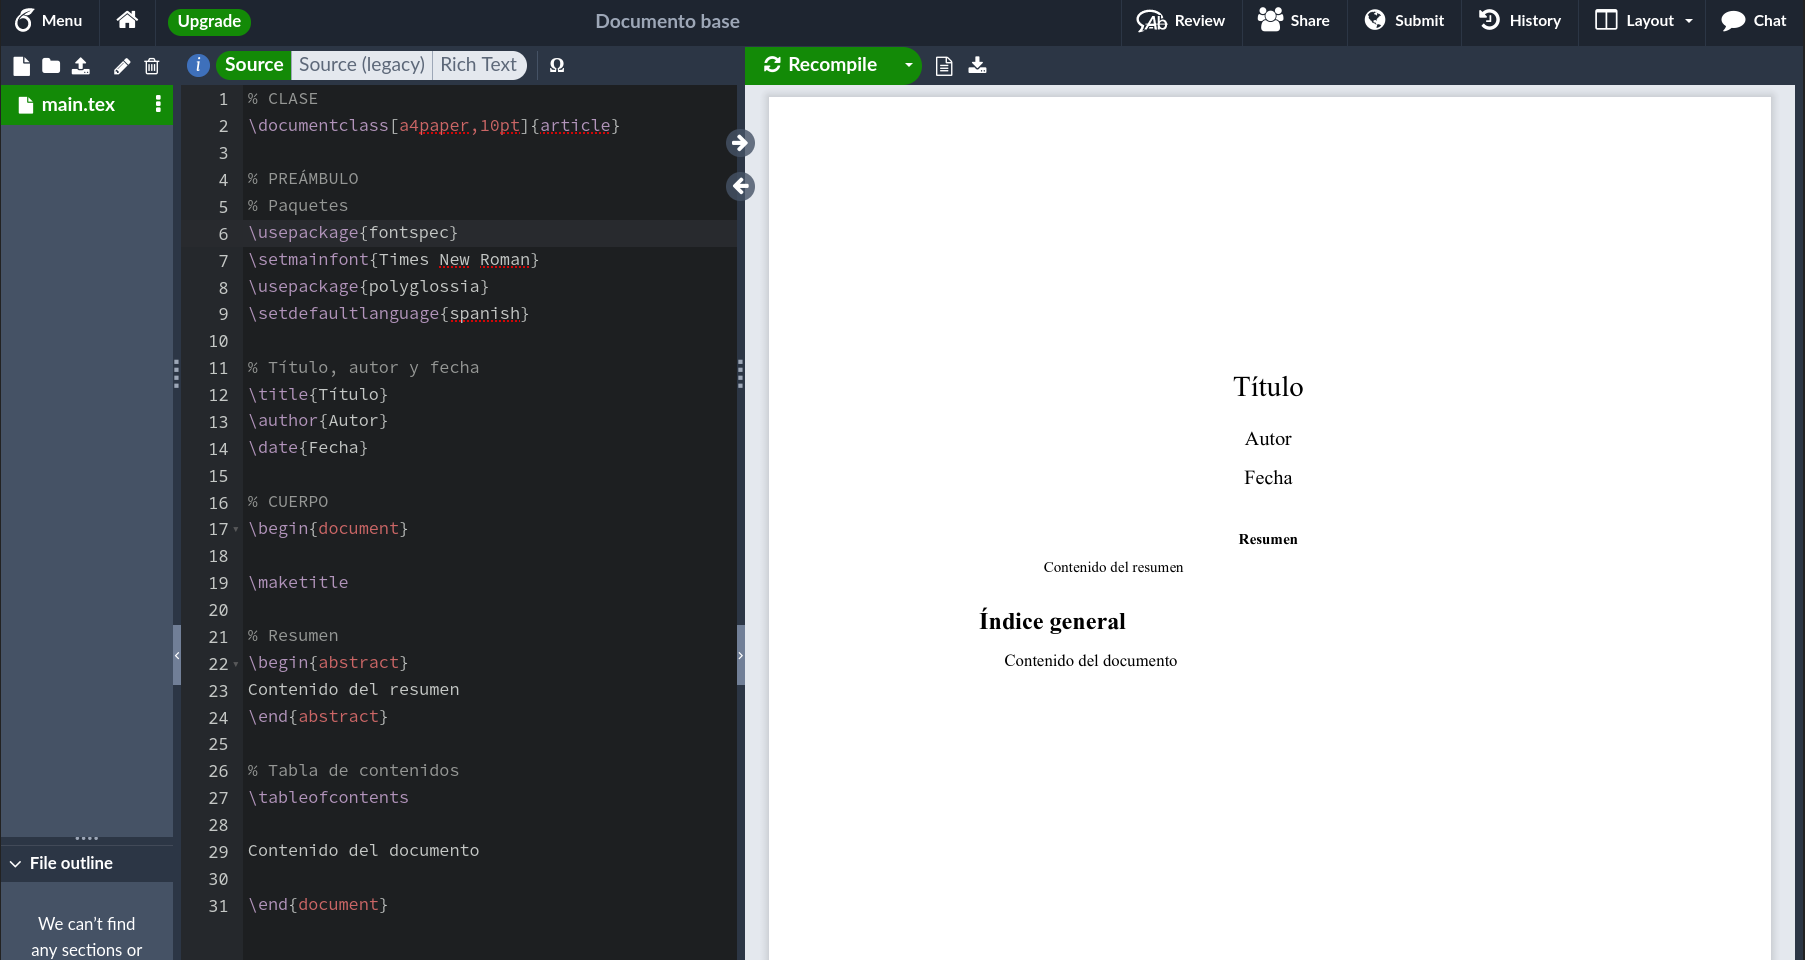
\includegraphics{./img/estructura/overleaf-documento-base.png}

}

\caption{\label{fig-overleaf-documento-base}Estructura básica de un
documento.}

\end{figure}

\bookmarksetup{startatroot}

\hypertarget{secciones-y-puxe1rrafos}{%
\chapter{Secciones y párrafos}\label{secciones-y-puxe1rrafos}}

\hypertarget{secciones-y-subsecciones}{%
\section{Secciones y subsecciones}\label{secciones-y-subsecciones}}

Normalmente un documento extenso se dividirá en secciones y subsecciones
(o incluso capítulos si se trata de un libro). Para definir las
secciones de un documento se utilizan los siguientes comandos:

\begin{itemize}
\tightlist
\item
  \texttt{\textbackslash{}chapter\{Título\ del\ capítulo\}}. Crea un
  nuevo capítulo con el título indicado y lo numera. Solo puede usarse
  cuando la clase del documento es \texttt{book}.
\item
  \texttt{\textbackslash{}section\{Título\ de\ la\ sección\}}. Crea una
  nueva sección con el título indicado y la numera.
\item
  \texttt{\textbackslash{}subsection\{Título\ de\ la\ subsección\}}.
  Crea una nueva subsección con el título indicado y la numera.
\item
  \texttt{\textbackslash{}subsubsection\{Título\ de\ la\ subsubsección\}}.
  Crea una nueva subsubsección con el título indicado y la numera.
\end{itemize}

Las secciones definidas con estos documentos aparecerán en la tabla de
contenidos automáticamente.

Existen versiones alternativas de estos comandos añadiendo un asterisco
(\texttt{\textbackslash{}chapter*}, \texttt{\textbackslash{}section*},
\texttt{\textbackslash{}subsection*},
\texttt{\textbackslash{}subsubsection*}) que crean encabezados de
sección sin numerar y que tampoco aparecerán en la tabla de contenidos.

\textbf{Ejemplo}

\begin{Shaded}
\begin{Highlighting}[]
\BuiltInTok{\textbackslash{}documentclass}\NormalTok{[a4paper, 10pt]\{}\ExtensionTok{article}\NormalTok{\}}
\NormalTok{...}
\CommentTok{\% CUERPO}
\KeywordTok{\textbackslash{}begin}\NormalTok{\{}\ExtensionTok{document}\NormalTok{\}}
\FunctionTok{\textbackslash{}tableofcontents}

\KeywordTok{\textbackslash{}section}\NormalTok{\{Sección primera\}}
\NormalTok{Texto de la sección.}

\KeywordTok{\textbackslash{}subsection}\NormalTok{\{Subsección primera\}}
\NormalTok{Texto de la subsección.}

\CommentTok{\% Encabezado de subsección sin numerar}
\KeywordTok{\textbackslash{}subsection*}\NormalTok{\{Subsección segunda\}}
\NormalTok{Texto de la subsección.}

\KeywordTok{\textbackslash{}subsection}\NormalTok{\{Subsección tercera\}}
\NormalTok{Texto de la subsección.}

\KeywordTok{\textbackslash{}section}\NormalTok{\{Sección segunda\}}
\NormalTok{Texto de la sección.}
\KeywordTok{\textbackslash{}end}\NormalTok{\{}\ExtensionTok{document}\NormalTok{\}}
\end{Highlighting}
\end{Shaded}

\begin{tcolorbox}[enhanced jigsaw, arc=.35mm, toprule=.15mm, opacitybacktitle=0.6, colback=white, coltitle=black, colbacktitle=quarto-callout-note-color!10!white, breakable, colframe=quarto-callout-note-color-frame, left=2mm, opacityback=0, bottomtitle=1mm, toptitle=1mm, titlerule=0mm, title={Salida}, bottomrule=.15mm, leftrule=.75mm, rightrule=.15mm]
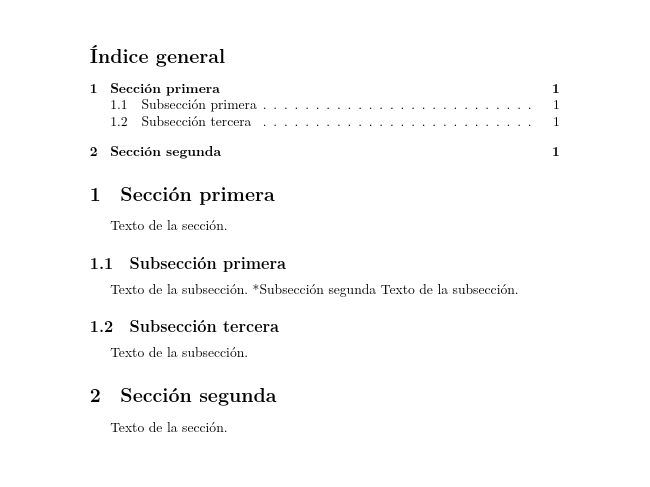
\includegraphics{./img/secciones/secciones.png}
\end{tcolorbox}

\hypertarget{puxe1rrafos-y-cambios-de-luxednea}{%
\section{Párrafos y cambios de
línea}\label{puxe1rrafos-y-cambios-de-luxednea}}

Para crear un párrafo nuevo basta dejar una o más líneas en blanco.

Si se quiere hacer un cambio de línea dentro de un mismo párrafo, se
utiliza el comando \texttt{\textbackslash{}newline} o
\texttt{\textbackslash{}\textbackslash{}}.

\textbf{Ejemplo}

\begin{Shaded}
\begin{Highlighting}[]
\CommentTok{\% CUERPO}
\KeywordTok{\textbackslash{}begin}\NormalTok{\{}\ExtensionTok{document}\NormalTok{\}}
\NormalTok{Este es el primer párrafo del documento, con un }\FunctionTok{\textbackslash{}\textbackslash{}}
\NormalTok{cambio de linea.}

\NormalTok{Este es el segundo párrafo del documento. Obsérvese que cada vez que se }
\NormalTok{comienza un párrafo la primera línea de desplaza un poco hacia la derecha. }
\NormalTok{Esto se conoce como }\FunctionTok{\textbackslash{}emph}\NormalTok{\{sangría\}.}
\KeywordTok{\textbackslash{}end}\NormalTok{\{}\ExtensionTok{document}\NormalTok{\}}
\end{Highlighting}
\end{Shaded}

\begin{tcolorbox}[enhanced jigsaw, arc=.35mm, toprule=.15mm, opacitybacktitle=0.6, colback=white, coltitle=black, colbacktitle=quarto-callout-note-color!10!white, breakable, colframe=quarto-callout-note-color-frame, left=2mm, opacityback=0, bottomtitle=1mm, toptitle=1mm, titlerule=0mm, title={Salida}, bottomrule=.15mm, leftrule=.75mm, rightrule=.15mm]
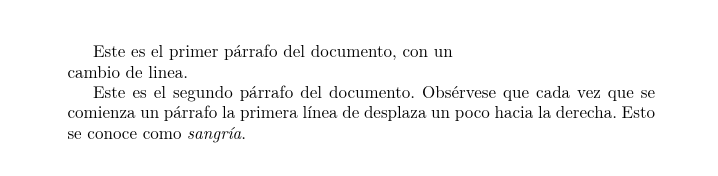
\includegraphics{./img/secciones/parrafos.png}
\end{tcolorbox}

\hypertarget{justificaciuxf3n}{%
\section{Justificación}\label{justificaciuxf3n}}

Los párrafos se justifican por defecto a la izquierda y a la derecha.
\LaTeX utiliza un algoritmo que permite partir las palabras al final
de una línea para obtener párrafos con una buena estética (sin grandes
espacios en blanco entre palabras). Pero también se pueden justificar
solo a la izquierda, solo a la derecha o centrados entre los márgenes.
Para ello se utilizan los siguientes entornos:

\begin{itemize}
\tightlist
\item
  \texttt{flushleft}: Justifica el texto a la izquierda.
\item
  \texttt{flushright}: Justifica el texto a la derecha.
\item
  \texttt{center}: Justifica el texto centrado entre los márgenes.
\end{itemize}

\begin{Shaded}
\begin{Highlighting}[]
\CommentTok{\% CUERPO}
\KeywordTok{\textbackslash{}begin}\NormalTok{\{}\ExtensionTok{document}\NormalTok{\}}
\NormalTok{Este es el primer párrafo del documento, y aparece justificado a ambos lados}
\NormalTok{(márgenes izquierdo y derecho) por defecto. Para que las líneas tengan la }
\NormalTok{misma longitud, se utiliza un algoritmo que permite partir las palabras al }
\NormalTok{final de una línea.}

\KeywordTok{\textbackslash{}begin}\NormalTok{\{}\ExtensionTok{flushleft}\NormalTok{\}}
\NormalTok{Este es el segundo párrafo del documento y aparece justificado a la }
\NormalTok{izquierda, es decir alineado con el margen izquierdo del documento. }
\NormalTok{Obsérvese que no todas las líneas acaban a la misma altura.}
\KeywordTok{\textbackslash{}end}\NormalTok{\{}\ExtensionTok{flushleft}\NormalTok{\}}

\KeywordTok{\textbackslash{}begin}\NormalTok{\{}\ExtensionTok{flushright}\NormalTok{\}}
\NormalTok{Este es el tercer párrafo del documento y aparece justificado a la derecha,}
\NormalTok{es decir alineado con el margen derecho del documento. Obsérvese que no }
\NormalTok{todas las líneas empiezan a la misma altura.}
\KeywordTok{\textbackslash{}end}\NormalTok{\{}\ExtensionTok{flushright}\NormalTok{\}}

\KeywordTok{\textbackslash{}begin}\NormalTok{\{}\ExtensionTok{center}\NormalTok{\}}
\NormalTok{Este es el último párrafo del documento y aparece justificado en el centro}
\NormalTok{entre los márgenes del documento. Obsérvese que ahora las líneas no }
\NormalTok{empiezan ni terminan a la misma altura. }
\KeywordTok{\textbackslash{}end}\NormalTok{\{}\ExtensionTok{center}\NormalTok{\}}
\KeywordTok{\textbackslash{}end}\NormalTok{\{}\ExtensionTok{document}\NormalTok{\}}
\end{Highlighting}
\end{Shaded}

\begin{tcolorbox}[enhanced jigsaw, arc=.35mm, toprule=.15mm, opacitybacktitle=0.6, colback=white, coltitle=black, colbacktitle=quarto-callout-note-color!10!white, breakable, colframe=quarto-callout-note-color-frame, left=2mm, opacityback=0, bottomtitle=1mm, toptitle=1mm, titlerule=0mm, title={Salida}, bottomrule=.15mm, leftrule=.75mm, rightrule=.15mm]
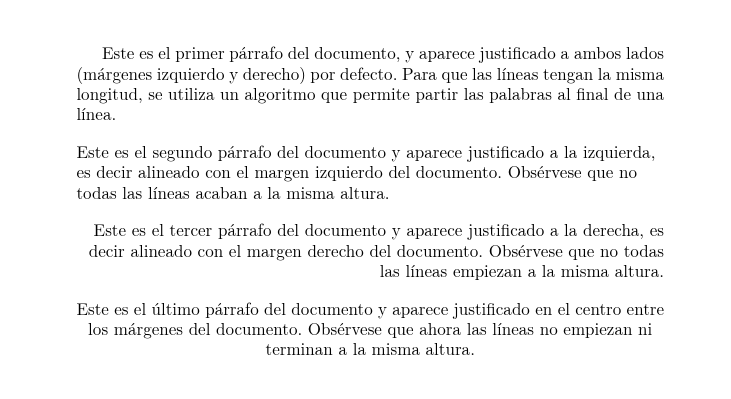
\includegraphics{./img/secciones/justificacion.png}
\end{tcolorbox}

\begin{tcolorbox}[enhanced jigsaw, arc=.35mm, toprule=.15mm, opacitybacktitle=0.6, colback=white, coltitle=black, colbacktitle=quarto-callout-warning-color!10!white, breakable, colframe=quarto-callout-warning-color-frame, left=2mm, opacityback=0, bottomtitle=1mm, toptitle=1mm, titlerule=0mm, title=\textcolor{quarto-callout-warning-color}{\faExclamationTriangle}\hspace{0.5em}{Advertencia}, bottomrule=.15mm, leftrule=.75mm, rightrule=.15mm]
El algoritmo para partir palabras al final de una línea funciona muy
bien, pero si alguna vez divide mal una palabra, se puede indicar por
dónde partir la palabra con el comando \texttt{\textbackslash{}-} (por
ejemplo \texttt{si\textbackslash{}-la\textbackslash{}-ba}).
\end{tcolorbox}

\bookmarksetup{startatroot}

\hypertarget{formateo-buxe1sico}{%
\chapter{Formateo básico}\label{formateo-buxe1sico}}

Existen multitud de comandos para dar formato al texto de un documento,
pero en esta sección nos limitaremos a los más importantes.

\hypertarget{negrita-cursiva-y-subrayado}{%
\section{Negrita, cursiva y
subrayado}\label{negrita-cursiva-y-subrayado}}

Para resaltar un texto habitualmente se utiliza negrita, cursiva o
subrayado. Estos formatos se aplican con los siguientes comandos:

\begin{itemize}
\tightlist
\item
  \texttt{\textbackslash{}textbf\{...\}}: Pone el texto en negrita.
\item
  \texttt{\textbackslash{}textit\{...\}}: Pone el texto en cursiva o
  itálica.
\item
  \texttt{\textbackslash{}emph\{...\}}: Enfatiza el texto cambiando de
  estilo (si estamos en un entorno de cursiva pasa a normal y si estamos
  en un entorno de texto normal pasa a cursiva).
\item
  \texttt{\textbackslash{}underline\{...\}}: Subraya el texto.
\end{itemize}

\textbf{Ejemplo}

\begin{Shaded}
\begin{Highlighting}[]
\CommentTok{\% CUERPO}
\KeywordTok{\textbackslash{}begin}\NormalTok{\{}\ExtensionTok{document}\NormalTok{\}}
\NormalTok{Este texto está en }\FunctionTok{\textbackslash{}textbf}\NormalTok{\{negrita\}, este en }\FunctionTok{\textbackslash{}textit}\NormalTok{\{cursiva\} y este }
\FunctionTok{\textbackslash{}underline}\NormalTok{\{subrayado\}. }

\FunctionTok{\textbackslash{}textit}\NormalTok{\{Este texto está }\FunctionTok{\textbackslash{}emph}\NormalTok{\{enfatizado\}\}.}
\KeywordTok{\textbackslash{}end}\NormalTok{\{}\ExtensionTok{document}\NormalTok{\}}
\end{Highlighting}
\end{Shaded}

\begin{tcolorbox}[enhanced jigsaw, arc=.35mm, toprule=.15mm, opacitybacktitle=0.6, colback=white, coltitle=black, colbacktitle=quarto-callout-note-color!10!white, breakable, colframe=quarto-callout-note-color-frame, left=2mm, opacityback=0, bottomtitle=1mm, toptitle=1mm, titlerule=0mm, title={Salida}, bottomrule=.15mm, leftrule=.75mm, rightrule=.15mm]
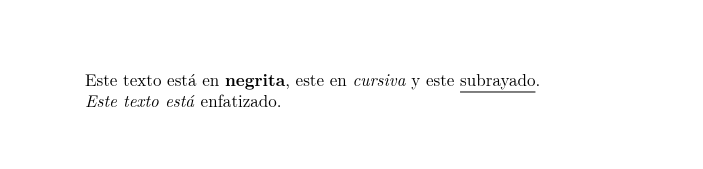
\includegraphics{./img/formateo/resaltado.png}
\end{tcolorbox}

\hypertarget{familias-de-tipos-de-letra}{%
\section{Familias de tipos de letra}\label{familias-de-tipos-de-letra}}

Existen tres tipos de letra que se activan con los siguientes comandos:

\begin{itemize}
\tightlist
\item
  \texttt{\textbackslash{}texrm\{...\}}: Texto normal (con
  \href{https://en.wikipedia.org/wiki/Serif}{serif}). Es el tipo por
  defecto.
\item
  \texttt{\textbackslash{}texsf\{...\}}: Texto sin adornos (sin serif)
\item
  \texttt{\textbackslash{}texttt\{...\}}: Texto de máquina de escribir o
  monoespaciado (caracteres con la misma anchura).
\end{itemize}

\textbf{Ejemplo}

\begin{Shaded}
\begin{Highlighting}[]
\CommentTok{\% CUERPO}
\KeywordTok{\textbackslash{}begin}\NormalTok{\{}\ExtensionTok{document}\NormalTok{\}}
\NormalTok{Este texto es normal, }\FunctionTok{\textbackslash{}textsf}\NormalTok{\{este es sin adornos\}, }\FunctionTok{\textbackslash{}texttt}\NormalTok{\{y este de máquina de escribir\}.}
\KeywordTok{\textbackslash{}end}\NormalTok{\{}\ExtensionTok{document}\NormalTok{\}}
\end{Highlighting}
\end{Shaded}

\begin{tcolorbox}[enhanced jigsaw, arc=.35mm, toprule=.15mm, opacitybacktitle=0.6, colback=white, coltitle=black, colbacktitle=quarto-callout-note-color!10!white, breakable, colframe=quarto-callout-note-color-frame, left=2mm, opacityback=0, bottomtitle=1mm, toptitle=1mm, titlerule=0mm, title={Salida}, bottomrule=.15mm, leftrule=.75mm, rightrule=.15mm]

\includegraphics{./img/formateo/tipos-letra.png}
\end{tcolorbox}

En el preámbulo del documento se puede seleccionar la fuente a utilizar
para cada uno de ellos, especialmente con el paquete \texttt{fontspec}
para compilar con \texttt{xelatex}. Para ello se utilizan los siguientes
comandos:

\begin{itemize}
\tightlist
\item
  \texttt{\textbackslash{}setromanfont\{Fuente\ normal\}}: Establece la
  fuente para el tipo de letra normal.
\item
  \texttt{\textbackslash{}setsansfont\{Fuente\ sin\ adorno\}}: Establece
  la fuente para el tipo de letra sin adorno.
\item
  \texttt{\textbackslash{}setmonofont\{Fuente\ monoespaciada\}}:
  Establece la fuente para el tipo de letra monoespaciado.
\end{itemize}

\begin{tcolorbox}[enhanced jigsaw, arc=.35mm, toprule=.15mm, opacitybacktitle=0.6, colback=white, coltitle=black, colbacktitle=quarto-callout-caution-color!10!white, breakable, colframe=quarto-callout-caution-color-frame, left=2mm, opacityback=0, bottomtitle=1mm, toptitle=1mm, titlerule=0mm, title=\textcolor{quarto-callout-caution-color}{\faFire}\hspace{0.5em}{Precaución}, bottomrule=.15mm, leftrule=.75mm, rightrule=.15mm]
Las fuentes utilizadas en un documento deben estar previamente
instaladas en el sistema operativo donde se compile el documento.
\end{tcolorbox}

\textbf{Ejemplo}

\begin{Shaded}
\begin{Highlighting}[]
\CommentTok{\% PREÁMBULO}
\BuiltInTok{\textbackslash{}usepackage}\NormalTok{\{}\ExtensionTok{fontspec}\NormalTok{\}}
\FunctionTok{\textbackslash{}setromanfont}\NormalTok{\{Times New Roman\}}
\FunctionTok{\textbackslash{}setsansfont}\NormalTok{\{Arial\}}
\FunctionTok{\textbackslash{}setmonofont}\NormalTok{\{Courier New\}}

\CommentTok{\% CUERPO}
\KeywordTok{\textbackslash{}begin}\NormalTok{\{}\ExtensionTok{document}\NormalTok{\}}
\NormalTok{Este texto es normal, }\FunctionTok{\textbackslash{}textsf}\NormalTok{\{este es sin adornos\}, }
\FunctionTok{\textbackslash{}texttt}\NormalTok{\{y este de máquina de escribir\}.}
\KeywordTok{\textbackslash{}end}\NormalTok{\{}\ExtensionTok{document}\NormalTok{\}}
\end{Highlighting}
\end{Shaded}

\begin{tcolorbox}[enhanced jigsaw, arc=.35mm, toprule=.15mm, opacitybacktitle=0.6, colback=white, coltitle=black, colbacktitle=quarto-callout-note-color!10!white, breakable, colframe=quarto-callout-note-color-frame, left=2mm, opacityback=0, bottomtitle=1mm, toptitle=1mm, titlerule=0mm, title={Salida}, bottomrule=.15mm, leftrule=.75mm, rightrule=.15mm]

\includegraphics{./img/formateo/tipos-letra-xelatex.png}
\end{tcolorbox}

\hypertarget{perfiles-de-letra}{%
\section{Perfiles de letra}\label{perfiles-de-letra}}

Para cada tipo de letra existen también varios perfiles que se activan
con los siguientes comandos:

\begin{itemize}
\tightlist
\item
  \texttt{\textbackslash{}textup\{...\}}: Activa el perfil recto. Es el
  perfil por defecto.
\item
  \texttt{\textbackslash{}textit\{...\}}: Activa el perfil de letra
  itálica.
\item
  \texttt{\textbackslash{}textsl\{...\}}: Activa el perfil inclinado.
\item
  \texttt{\textbackslash{}textsc\{...\}}: Activa el perfil de letra
  versalita (mayúsculas pequeñas).
\end{itemize}

\textbf{Ejemplo}

\begin{Shaded}
\begin{Highlighting}[]
\CommentTok{\% CUERPO}
\KeywordTok{\textbackslash{}begin}\NormalTok{\{}\ExtensionTok{document}\NormalTok{\}}
\NormalTok{Texto normal con perfil recto, }\FunctionTok{\textbackslash{}textit}\NormalTok{\{itálica\}, }\FunctionTok{\textbackslash{}textsl}\NormalTok{\{inclinado\} y }
\FunctionTok{\textbackslash{}textsc}\NormalTok{\{versalita\}.}

\FunctionTok{\textbackslash{}textsf}\NormalTok{\{Texto sin adorno con perfil recto, }\FunctionTok{\textbackslash{}textit}\NormalTok{\{itálica\}, }
\FunctionTok{\textbackslash{}textsl}\NormalTok{\{inclinado\} y }\FunctionTok{\textbackslash{}textsc}\NormalTok{\{versalita\}.\}}

\FunctionTok{\textbackslash{}texttt}\NormalTok{\{Texto monoespaciado con perfil recto, }\FunctionTok{\textbackslash{}textit}\NormalTok{\{itálica\}, }
\FunctionTok{\textbackslash{}textsl}\NormalTok{\{inclinado\} y }\FunctionTok{\textbackslash{}textsc}\NormalTok{\{versalita\}.\}}
\KeywordTok{\textbackslash{}end}\NormalTok{\{}\ExtensionTok{document}\NormalTok{\}}
\end{Highlighting}
\end{Shaded}

\begin{tcolorbox}[enhanced jigsaw, arc=.35mm, toprule=.15mm, opacitybacktitle=0.6, colback=white, coltitle=black, colbacktitle=quarto-callout-note-color!10!white, breakable, colframe=quarto-callout-note-color-frame, left=2mm, opacityback=0, bottomtitle=1mm, toptitle=1mm, titlerule=0mm, title={Salida}, bottomrule=.15mm, leftrule=.75mm, rightrule=.15mm]
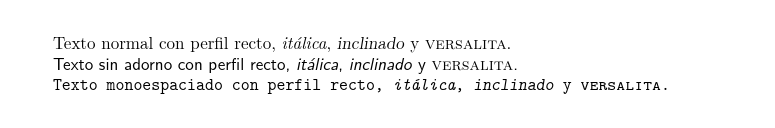
\includegraphics{./img/formateo/perfiles-letra.png}
\end{tcolorbox}

\hypertarget{tamauxf1os-de-letra}{%
\section{Tamaños de letra}\label{tamauxf1os-de-letra}}

A diferencia de otros procesadores donde el tamaño de la fuente se
indica en puntos o pixels, en \LaTeX existen 10 tamaños predefinidos
que se activan con los siguientes comandos, de menor a mayor tamaño:

\begin{itemize}
\tightlist
\item
  \texttt{\textbackslash{}tiny}
\item
  \texttt{\textbackslash{}scriptsize}
\item
  \texttt{\textbackslash{}footnotesize}
\item
  \texttt{\textbackslash{}small}
\item
  \texttt{\textbackslash{}normalsize}
\item
  \texttt{\textbackslash{}large}
\item
  \texttt{\textbackslash{}Large}
\item
  \texttt{\textbackslash{}LARGE}
\item
  \texttt{\textbackslash{}huge}
\item
  \texttt{\textbackslash{}Huge}
\end{itemize}

Existen paquetes que permiten definir tamaños más pequeños o mayores
pero no suelen ser necesarios en un documento normal.

\textbf{Ejemplo}

\begin{Shaded}
\begin{Highlighting}[]
\CommentTok{\% CUERPO}
\KeywordTok{\textbackslash{}begin}\NormalTok{\{}\ExtensionTok{document}\NormalTok{\}}
\FunctionTok{\textbackslash{}tiny}\NormalTok{\{tiny\}}
\FunctionTok{\textbackslash{}scriptsize}\NormalTok{\{scripsize\} }
\FunctionTok{\textbackslash{}footnotesize}\NormalTok{\{footnotesize\}}
\FunctionTok{\textbackslash{}small}\NormalTok{\{small\}}
\FunctionTok{\textbackslash{}normalsize}\NormalTok{\{normalsize\}}
\FunctionTok{\textbackslash{}large}\NormalTok{\{large\} }
\FunctionTok{\textbackslash{}Large}\NormalTok{\{Large\}}
\FunctionTok{\textbackslash{}LARGE}\NormalTok{\{LARGE\}}
\FunctionTok{\textbackslash{}huge}\NormalTok{\{huge\}}
\FunctionTok{\textbackslash{}Huge}\NormalTok{\{Huge\}}
\KeywordTok{\textbackslash{}end}\NormalTok{\{}\ExtensionTok{document}\NormalTok{\}}
\end{Highlighting}
\end{Shaded}

\begin{tcolorbox}[enhanced jigsaw, arc=.35mm, toprule=.15mm, opacitybacktitle=0.6, colback=white, coltitle=black, colbacktitle=quarto-callout-note-color!10!white, breakable, colframe=quarto-callout-note-color-frame, left=2mm, opacityback=0, bottomtitle=1mm, toptitle=1mm, titlerule=0mm, title={Salida}, bottomrule=.15mm, leftrule=.75mm, rightrule=.15mm]
\includegraphics{./img/formateo/tamaño-fuente.png}
\end{tcolorbox}

\bookmarksetup{startatroot}

\hypertarget{listas}{%
\chapter{Listas}\label{listas}}

Existen tres tipos de listas, no ordenadas, ordenadas y descriptivas (en
lugar de marcas o números los items de la lista están encabezados por
texto), que se crean con los siguientes entornos:

\begin{itemize}
\tightlist
\item
  \texttt{itemize}: Crea un lista sin numerar.
\item
  \texttt{enumerate}: Crea una lista enumerada.
\item
  \texttt{description}: Crea una lista de tipo descripción.
\end{itemize}

Dentro de estos entornos, cada elemento de la lista debe empezar en una
línea nueva con el comando \texttt{\textbackslash{}item}. En el caso de
las listas descriptivas, hay que proporcionar el texto del item de la
lista como un argumento obligatorio.

\textbf{Ejemplos}

Ejemplo de lista no ordenada.

\begin{Shaded}
\begin{Highlighting}[]
\CommentTok{\% CUERPO}
\KeywordTok{\textbackslash{}begin}\NormalTok{\{}\ExtensionTok{document}\NormalTok{\}}
\NormalTok{Ejemplo de lista no ordenada:}
\KeywordTok{\textbackslash{}begin}\NormalTok{\{}\ExtensionTok{itemize}\NormalTok{\}}
\FunctionTok{\textbackslash{}item}\NormalTok{ Este es un item.}
\FunctionTok{\textbackslash{}item}\NormalTok{ Este es otro item.}
\FunctionTok{\textbackslash{}item}\NormalTok{ Y otro item más.}
\KeywordTok{\textbackslash{}end}\NormalTok{\{}\ExtensionTok{itemize}\NormalTok{\}}
\KeywordTok{\textbackslash{}end}\NormalTok{\{}\ExtensionTok{document}\NormalTok{\}}
\end{Highlighting}
\end{Shaded}

\begin{tcolorbox}[enhanced jigsaw, arc=.35mm, toprule=.15mm, opacitybacktitle=0.6, colback=white, coltitle=black, colbacktitle=quarto-callout-note-color!10!white, breakable, colframe=quarto-callout-note-color-frame, left=2mm, opacityback=0, bottomtitle=1mm, toptitle=1mm, titlerule=0mm, title={Salida}, bottomrule=.15mm, leftrule=.75mm, rightrule=.15mm]

\includegraphics{./img/listas/lista-no-ordenad.png}
\end{tcolorbox}

Ejemplo de lista ordenada.

\begin{Shaded}
\begin{Highlighting}[]
\CommentTok{\% CUERPO}
\KeywordTok{\textbackslash{}begin}\NormalTok{\{}\ExtensionTok{document}\NormalTok{\}}
\NormalTok{Ejemplo de lista ordenada:}
\KeywordTok{\textbackslash{}begin}\NormalTok{\{}\ExtensionTok{enumerate}\NormalTok{\}}
\FunctionTok{\textbackslash{}item}\NormalTok{ Primer item.}
\FunctionTok{\textbackslash{}item}\NormalTok{ Segundo item.}
\FunctionTok{\textbackslash{}item}\NormalTok{ Tercer item.}
\KeywordTok{\textbackslash{}end}\NormalTok{\{}\ExtensionTok{enumerate}\NormalTok{\}}
\KeywordTok{\textbackslash{}end}\NormalTok{\{}\ExtensionTok{document}\NormalTok{\}}
\end{Highlighting}
\end{Shaded}

\begin{tcolorbox}[enhanced jigsaw, arc=.35mm, toprule=.15mm, opacitybacktitle=0.6, colback=white, coltitle=black, colbacktitle=quarto-callout-note-color!10!white, breakable, colframe=quarto-callout-note-color-frame, left=2mm, opacityback=0, bottomtitle=1mm, toptitle=1mm, titlerule=0mm, title={Salida}, bottomrule=.15mm, leftrule=.75mm, rightrule=.15mm]
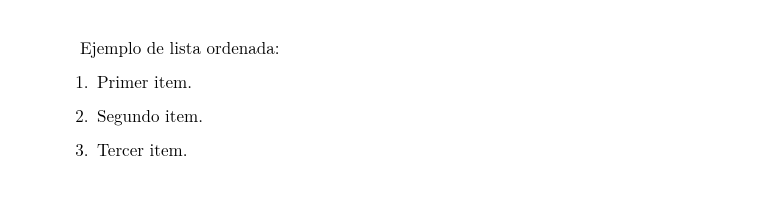
\includegraphics{./img/listas/lista-ordenada.png}
\end{tcolorbox}

Ejemplo de lista descriptiva.

\begin{Shaded}
\begin{Highlighting}[]
\CommentTok{\% CUERPO}
\KeywordTok{\textbackslash{}begin}\NormalTok{\{}\ExtensionTok{document}\NormalTok{\}}
\NormalTok{Ejemplo de lista descriptiva:}
\KeywordTok{\textbackslash{}begin}\NormalTok{\{}\ExtensionTok{description}\NormalTok{\}}
\FunctionTok{\textbackslash{}item}\NormalTok{\{}\FunctionTok{\textbackslash{}textbf}\NormalTok{\{latex\}\} Genera documentos en formato dvi.}
\FunctionTok{\textbackslash{}item}\NormalTok{\{}\FunctionTok{\textbackslash{}textbf}\NormalTok{\{pdflatex\}\} Genera documentos en formato pdf.}
\FunctionTok{\textbackslash{}item}\NormalTok{\{}\FunctionTok{\textbackslash{}textbf}\NormalTok{\{xelatex\}\} Genera documentos en formato pdf que admiten }
\NormalTok{codificación Unicode.}
\KeywordTok{\textbackslash{}end}\NormalTok{\{}\ExtensionTok{description}\NormalTok{\}}
\KeywordTok{\textbackslash{}end}\NormalTok{\{}\ExtensionTok{document}\NormalTok{\}}
\end{Highlighting}
\end{Shaded}

\begin{tcolorbox}[enhanced jigsaw, arc=.35mm, toprule=.15mm, opacitybacktitle=0.6, colback=white, coltitle=black, colbacktitle=quarto-callout-note-color!10!white, breakable, colframe=quarto-callout-note-color-frame, left=2mm, opacityback=0, bottomtitle=1mm, toptitle=1mm, titlerule=0mm, title={Salida}, bottomrule=.15mm, leftrule=.75mm, rightrule=.15mm]

\includegraphics{./img/listas/lista-desciptiva.png}
\end{tcolorbox}

Se pueden crear sublistas anidando unos entornos dentro de otros.

\textbf{Ejemplo}

\begin{Shaded}
\begin{Highlighting}[]
\CommentTok{\% CUERPO}
\KeywordTok{\textbackslash{}begin}\NormalTok{\{}\ExtensionTok{document}\NormalTok{\}}
\NormalTok{Ejemplo de listas anidadas:}
\KeywordTok{\textbackslash{}begin}\NormalTok{\{}\ExtensionTok{enumerate}\NormalTok{\}}
\FunctionTok{\textbackslash{}item}\NormalTok{ Primer item.}
    \KeywordTok{\textbackslash{}begin}\NormalTok{\{}\ExtensionTok{enumerate}\NormalTok{\}}
    \FunctionTok{\textbackslash{}item}\NormalTok{ Primer subitem.}
    \FunctionTok{\textbackslash{}item}\NormalTok{ Segundo subitem.}
    \KeywordTok{\textbackslash{}end}\NormalTok{\{}\ExtensionTok{enumerate}\NormalTok{\}}
\FunctionTok{\textbackslash{}item}\NormalTok{ Segundo item.}
    \KeywordTok{\textbackslash{}begin}\NormalTok{\{}\ExtensionTok{itemize}\NormalTok{\}}
    \FunctionTok{\textbackslash{}item}\NormalTok{ Un item.}
    \FunctionTok{\textbackslash{}item}\NormalTok{ Otro item.}
    \KeywordTok{\textbackslash{}end}\NormalTok{\{}\ExtensionTok{itemize}\NormalTok{\}}
\KeywordTok{\textbackslash{}end}\NormalTok{\{}\ExtensionTok{enumerate}\NormalTok{\}}
\KeywordTok{\textbackslash{}end}\NormalTok{\{}\ExtensionTok{document}\NormalTok{\}}
\end{Highlighting}
\end{Shaded}

\begin{tcolorbox}[enhanced jigsaw, arc=.35mm, toprule=.15mm, opacitybacktitle=0.6, colback=white, coltitle=black, colbacktitle=quarto-callout-note-color!10!white, breakable, colframe=quarto-callout-note-color-frame, left=2mm, opacityback=0, bottomtitle=1mm, toptitle=1mm, titlerule=0mm, title={Salida}, bottomrule=.15mm, leftrule=.75mm, rightrule=.15mm]
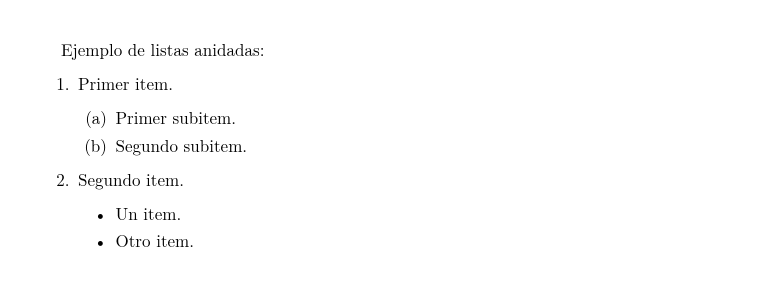
\includegraphics{./img/listas/listas-anidadas.png}
\end{tcolorbox}

La indentación en el código fuente del ejemplo anterior no es
obligatoria pero ayuda a ver mejor la estructura de anidamiento de
entornos.

\bookmarksetup{startatroot}

\hypertarget{sec-tablas}{%
\chapter{Tablas}\label{sec-tablas}}

Las tablas son uno de los elementos más complejos de \LaTeX, ya que,
aunque es fácil crear una tabla sencilla, aplicarles un formato más
avanzado con justificación de columnas, fusión de columnas o filas,
márgenes de columnas, líneas de división, etc. suele ser bastante más
difícil, aunque algunos entornos de edición facilitan la tarea. Existen
multitud de paquetes para personalizar las tablas pero en esta sección
solo veremos lo más básico.

Para crear una tabla se utiliza el entorno \texttt{tabular}. Este
entorno tiene como argumento obligatorio el número de columnas de la
tabla y su justificación, que se indica con una letra: \texttt{l}
izquierda, \texttt{r} derecha y \texttt{c} centrada, (por ejemplo
\texttt{lcr} indica tres columnas, la primera justificada a la
izquierda, la segunda centrada y la tercera justificada a la derecha).

A continuación se introduce el contenido de la tabla, separando las
filas con el comando de cambio de línea
\texttt{\textbackslash{}\textbackslash{}} y dentro de cada línea
separando las celdas con el comando \texttt{\&}.

\textbf{Ejemplo}

\begin{Shaded}
\begin{Highlighting}[]
\CommentTok{\% CUERPO}
\KeywordTok{\textbackslash{}begin}\NormalTok{\{}\ExtensionTok{document}\NormalTok{\}}
\CommentTok{\% Tabla con tres columnas, justificadas a la izquierda, centrada y derecha.}
\KeywordTok{\textbackslash{}begin}\NormalTok{\{}\ExtensionTok{tabular}\NormalTok{\}\{lcr\}}
\NormalTok{Nombre }\OperatorTok{\&}\NormalTok{ Ciudad }\OperatorTok{\&}\NormalTok{ Edad }\FunctionTok{\textbackslash{}\textbackslash{}}
\NormalTok{María }\OperatorTok{\&}\NormalTok{ Valencia }\OperatorTok{\&}\NormalTok{ 22 }\FunctionTok{\textbackslash{}\textbackslash{}}
\NormalTok{Juan }\OperatorTok{\&}\NormalTok{ Madrid }\OperatorTok{\&}\NormalTok{ 50 }\FunctionTok{\textbackslash{}\textbackslash{}}
\NormalTok{Carmen }\OperatorTok{\&}\NormalTok{ Barcelona }\OperatorTok{\&}\NormalTok{ 35 }\FunctionTok{\textbackslash{}\textbackslash{}}
\KeywordTok{\textbackslash{}end}\NormalTok{\{}\ExtensionTok{tabular}\NormalTok{\}}
\KeywordTok{\textbackslash{}end}\NormalTok{\{}\ExtensionTok{document}\NormalTok{\}}
\end{Highlighting}
\end{Shaded}

\begin{tcolorbox}[enhanced jigsaw, arc=.35mm, toprule=.15mm, opacitybacktitle=0.6, colback=white, coltitle=black, colbacktitle=quarto-callout-note-color!10!white, breakable, colframe=quarto-callout-note-color-frame, left=2mm, opacityback=0, bottomtitle=1mm, toptitle=1mm, titlerule=0mm, title={Salida}, bottomrule=.15mm, leftrule=.75mm, rightrule=.15mm]

\includegraphics{./img/tablas/tabla-simple.png}
\end{tcolorbox}

Para añadir líneas de división entre columnas, se introduce el carácter
de barra vertical \texttt{\textbar{}} entre las letras que definen la
justificación de las columnas en el argumento obligatorio del entorno
\texttt{tabular}. Mientras que para añadir líneas de división entre
filas, se utiliza el comando \texttt{\textbackslash{}hline} al principio
de cada línea. Se insertarán tantas líneas divisorias como veces se
introduzca el comando \texttt{\textbackslash{}hline}.

\textbf{Ejemplo}

\begin{Shaded}
\begin{Highlighting}[]
\CommentTok{\% CUERPO}
\KeywordTok{\textbackslash{}begin}\NormalTok{\{}\ExtensionTok{document}\NormalTok{\}}
\CommentTok{\% Tabla con líneas divisorias de filas y columnas.}
\KeywordTok{\textbackslash{}begin}\NormalTok{\{}\ExtensionTok{tabular}\NormalTok{\}\{|l|c|r|\}}
\FunctionTok{\textbackslash{}hline}
\NormalTok{Nombre }\OperatorTok{\&}\NormalTok{ Ciudad }\OperatorTok{\&}\NormalTok{ Edad }\FunctionTok{\textbackslash{}\textbackslash{}} 
\FunctionTok{\textbackslash{}hline}
\FunctionTok{\textbackslash{}hline}
\NormalTok{María }\OperatorTok{\&}\NormalTok{ Valencia }\OperatorTok{\&}\NormalTok{ 22 }\FunctionTok{\textbackslash{}\textbackslash{}}
\FunctionTok{\textbackslash{}hline}
\NormalTok{Juan }\OperatorTok{\&}\NormalTok{ Madrid }\OperatorTok{\&}\NormalTok{ 50 }\FunctionTok{\textbackslash{}\textbackslash{}}
\FunctionTok{\textbackslash{}hline}
\NormalTok{Carmen }\OperatorTok{\&}\NormalTok{ Barcelona }\OperatorTok{\&}\NormalTok{ 35 }\FunctionTok{\textbackslash{}\textbackslash{}}
\FunctionTok{\textbackslash{}hline}
\KeywordTok{\textbackslash{}end}\NormalTok{\{}\ExtensionTok{tabular}\NormalTok{\}}
\KeywordTok{\textbackslash{}end}\NormalTok{\{}\ExtensionTok{document}\NormalTok{\}}
\end{Highlighting}
\end{Shaded}

\begin{tcolorbox}[enhanced jigsaw, arc=.35mm, toprule=.15mm, opacitybacktitle=0.6, colback=white, coltitle=black, colbacktitle=quarto-callout-note-color!10!white, breakable, colframe=quarto-callout-note-color-frame, left=2mm, opacityback=0, bottomtitle=1mm, toptitle=1mm, titlerule=0mm, title={Salida}, bottomrule=.15mm, leftrule=.75mm, rightrule=.15mm]
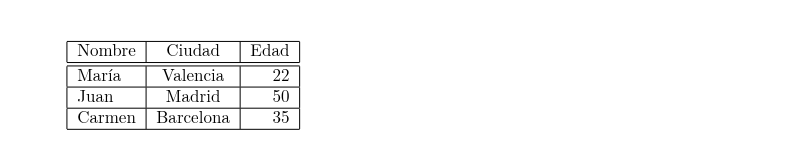
\includegraphics{./img/tablas/tabla-delimitada.png}
\end{tcolorbox}

El comando \texttt{\textbackslash{}multicolumn\{num\}\{col\}\{texto\}}
permite crear celdas que se extienden a lo largo de varias columnas,
donde \texttt{num} es el número de columnas a ocupar, \texttt{col} es el
carácter que define la justificación de la celda (\texttt{l}, \texttt{r}
o \texttt{c}), y \texttt{texto} es el contenido de la celda.

También es posible utilizar el comando
\texttt{\textbackslash{}cline\{n-m\}} para dibujar líneas horizontales
divisorias que no abarquen toda la fila, sino desde la columna
\texttt{n} hasta la \texttt{m}.

\textbf{Ejemplo}

\begin{Shaded}
\begin{Highlighting}[]
\CommentTok{\% CUERPO}
\KeywordTok{\textbackslash{}begin}\NormalTok{\{}\ExtensionTok{document}\NormalTok{\}}
\KeywordTok{\textbackslash{}begin}\NormalTok{\{}\ExtensionTok{tabular}\NormalTok{\}\{lrrcrr\}}
\FunctionTok{\textbackslash{}hline}
 \OperatorTok{\&} \FunctionTok{\textbackslash{}multicolumn}\NormalTok{\{2\}\{c\}\{Enero\} }\OperatorTok{\&} \OperatorTok{\&} \FunctionTok{\textbackslash{}multicolumn}\NormalTok{\{2\}\{c\}\{Febrero\}}\FunctionTok{\textbackslash{}\textbackslash{}}
\FunctionTok{\textbackslash{}cline}\NormalTok{\{2{-}3\}}\FunctionTok{\textbackslash{}cline}\NormalTok{\{5{-}6\}}
\NormalTok{Ciudad }\OperatorTok{\&}\NormalTok{ Ingresos }\OperatorTok{\&}\NormalTok{ Gastos }\OperatorTok{\&} \OperatorTok{\&}\NormalTok{ Ingresos }\OperatorTok{\&}\NormalTok{ Gastos}\FunctionTok{\textbackslash{}\textbackslash{}} 
\FunctionTok{\textbackslash{}hline}
\NormalTok{Madrid }\OperatorTok{\&}\NormalTok{ 2500 }\OperatorTok{\&}\NormalTok{ 1750 }\OperatorTok{\&} \OperatorTok{\&}\NormalTok{ 2600 }\OperatorTok{\&}\NormalTok{ 1800}\FunctionTok{\textbackslash{}\textbackslash{}} 
\NormalTok{Barcelona }\OperatorTok{\&}\NormalTok{ 2250 }\OperatorTok{\&}\NormalTok{ 1500 }\OperatorTok{\&} \OperatorTok{\&}\NormalTok{ 2400 }\OperatorTok{\&}\NormalTok{ 1650}\FunctionTok{\textbackslash{}\textbackslash{}} 
\FunctionTok{\textbackslash{}hline}
\KeywordTok{\textbackslash{}end}\NormalTok{\{}\ExtensionTok{tabular}\NormalTok{\}}
\KeywordTok{\textbackslash{}end}\NormalTok{\{}\ExtensionTok{document}\NormalTok{\}}
\end{Highlighting}
\end{Shaded}

\begin{tcolorbox}[enhanced jigsaw, arc=.35mm, toprule=.15mm, opacitybacktitle=0.6, colback=white, coltitle=black, colbacktitle=quarto-callout-note-color!10!white, breakable, colframe=quarto-callout-note-color-frame, left=2mm, opacityback=0, bottomtitle=1mm, toptitle=1mm, titlerule=0mm, title={Salida}, bottomrule=.15mm, leftrule=.75mm, rightrule=.15mm]
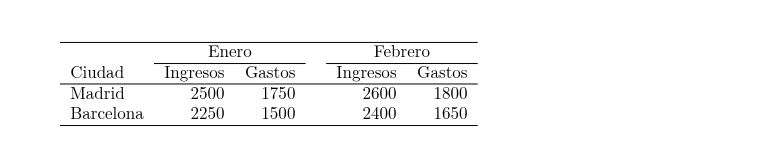
\includegraphics{./img/tablas/tabla-multicolumna.png}
\end{tcolorbox}

\bookmarksetup{startatroot}

\hypertarget{imuxe1genes}{%
\chapter{Imágenes}\label{imuxe1genes}}

Para incluir una imagen o figura en un documento, además de disponer de
la imagen del fichero en un formato gráfico adecuado, es necesario
cargar en el preámbulo el paquete \texttt{graphicx}. Este paquete
permite gestionar imágenes en los formatos gráficos \texttt{jpg},
\texttt{png}, \texttt{tiff}, \texttt{eps} y \texttt{pdf} (los tres
primeros son formatos de mapas de bits y los dos últimos vectoriales).

Una vez cargado el paquete, para insertar una imagen en el documento
basta con utilizar el comando
\texttt{\textbackslash{}includegraphics{[}opiones{]}\{fichero\}}. Este
comando tiene como argumento obligatorio es el nombre del fichero con la
imagen (incluyendo la ruta en el sistema de ficheros local) y los
siguientes argumentos opcionales para modificar el aspecto de la imagen:

\begin{itemize}
\tightlist
\item
  \texttt{height}: Indica la altura de la imagen. Escala la imagen hasta
  esa altura.
\item
  \texttt{width}: Indica la anchura de la imagen. Escala la imagen hasta
  esa anchura.
\item
  \texttt{scale}: Factor de escalado de la imagen de 0 a 1.
\item
  \texttt{angle}: Ángulo de rotación de la imagen. Rota la imagen en el
  sentido de las agujas del reloj los grados indicados.
\end{itemize}

\textbf{Ejemplo}

\begin{Shaded}
\begin{Highlighting}[]
\CommentTok{\% PREÁMBULO}
\BuiltInTok{\textbackslash{}usepackage}\NormalTok{\{}\ExtensionTok{graphicx}\NormalTok{\}}
\CommentTok{\% CUERPO}
\KeywordTok{\textbackslash{}begin}\NormalTok{\{}\ExtensionTok{document}\NormalTok{\}}
\NormalTok{Ejemplo de imagen en línea }
\BuiltInTok{\textbackslash{}includegraphics}\NormalTok{\{}\ExtensionTok{img/logo{-}aprendeconalf.png}\NormalTok{\}, }
\NormalTok{escalada}
\BuiltInTok{\textbackslash{}includegraphics}\NormalTok{[height=1cm]\{}\ExtensionTok{img/logo{-}aprendeconalf.png}\NormalTok{\},}
\NormalTok{y rotada}
\BuiltInTok{\textbackslash{}includegraphics}\NormalTok{[angle=90]\{}\ExtensionTok{img/logo{-}aprendeconalf.png}\NormalTok{\}}

\NormalTok{Ejemplo de imagen centrada:}

\KeywordTok{\textbackslash{}begin}\NormalTok{\{}\ExtensionTok{center}\NormalTok{\}}
\BuiltInTok{\textbackslash{}includegraphics}\NormalTok{\{}\ExtensionTok{img/logo{-}aprendeconalf.png}\NormalTok{\}}
\KeywordTok{\textbackslash{}end}\NormalTok{\{}\ExtensionTok{center}\NormalTok{\}}
\KeywordTok{\textbackslash{}end}\NormalTok{\{}\ExtensionTok{document}\NormalTok{\}}
\end{Highlighting}
\end{Shaded}

\begin{tcolorbox}[enhanced jigsaw, arc=.35mm, toprule=.15mm, opacitybacktitle=0.6, colback=white, coltitle=black, colbacktitle=quarto-callout-note-color!10!white, breakable, colframe=quarto-callout-note-color-frame, left=2mm, opacityback=0, bottomtitle=1mm, toptitle=1mm, titlerule=0mm, title={Salida}, bottomrule=.15mm, leftrule=.75mm, rightrule=.15mm]

\includegraphics{./img/imagenes/imganes.png}
\end{tcolorbox}

\bookmarksetup{startatroot}

\hypertarget{fuxf3rmulas-matemuxe1ticas}{%
\chapter{Fórmulas matemáticas}\label{fuxf3rmulas-matemuxe1ticas}}

La escritura de fórmulas matemáticas es uno de los puntos fuertes de
\LaTeX, y es por ello que se utiliza tanto para la creación de
documentos científicos o técnicos con contenido matemático.

Para escribir una fórmula es necesario cambiar al modo matemático.
Existen distintas formas de activar el modo matemático:

\begin{itemize}
\item
  \texttt{\$}: Activa el modo matemático en linea, es decir, las
  fórmulas aparecerán en la misma linea que el texto que las rodea. Para
  desactivar este modo hay que volver a escriri \texttt{\$}.
\item
  \texttt{\$\$}: Activa el modo matemático \emph{display} (desplegado),
  de manera que las fórmulas aparecen en una línea aparte.
\item
  El entorno \texttt{equation} también activa el modo matemático
  \emph{display} pero además asigna un número a la ecuación, para poder
  referenciarla en otras partes del documento.
\end{itemize}

\textbf{Ejemplo}

\begin{Shaded}
\begin{Highlighting}[]
\CommentTok{\% CUERPO}
\KeywordTok{\textbackslash{}begin}\NormalTok{\{}\ExtensionTok{document}\NormalTok{\}}
\NormalTok{Ejemplo de fórmula en linea }\SpecialStringTok{$ x+y=0 $}\NormalTok{.}

\NormalTok{Ejemplo de fórmula desplegada}

\SpecialStringTok{$$ }
\SpecialStringTok{x+y=0}
\SpecialStringTok{$$}



\NormalTok{Ejemplo de fórmula con el entorno }\FunctionTok{\textbackslash{}texttt}\NormalTok{\{equation\}}

\KeywordTok{\textbackslash{}begin}\NormalTok{\{}\ExtensionTok{equation}\NormalTok{\}}
\SpecialStringTok{x+y=0}
\KeywordTok{\textbackslash{}end}\NormalTok{\{}\ExtensionTok{equation}\NormalTok{\}}
\KeywordTok{\textbackslash{}end}\NormalTok{\{}\ExtensionTok{document}\NormalTok{\}}
\end{Highlighting}
\end{Shaded}

\begin{tcolorbox}[enhanced jigsaw, arc=.35mm, toprule=.15mm, opacitybacktitle=0.6, colback=white, coltitle=black, colbacktitle=quarto-callout-note-color!10!white, breakable, colframe=quarto-callout-note-color-frame, left=2mm, opacityback=0, bottomtitle=1mm, toptitle=1mm, titlerule=0mm, title={Salida}, bottomrule=.15mm, leftrule=.75mm, rightrule=.15mm]
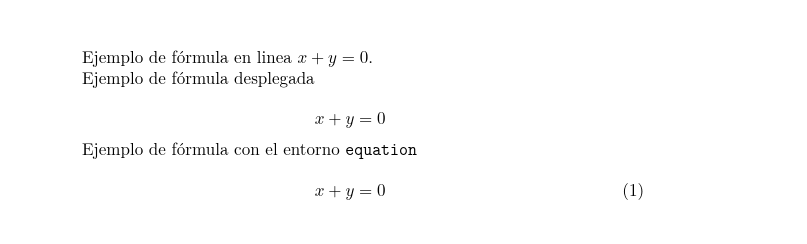
\includegraphics{./img/formulas/entornos-matematicos.png}
\end{tcolorbox}

\hypertarget{suxedmbolos-matemuxe1ticos}{%
\section{Símbolos matemáticos}\label{suxedmbolos-matemuxe1ticos}}

Existe una infinidad de símbolos matemáticos que escriben mediante
comandos. A continuación se muestran los más habituales.\footnote{Para
  un listado más exhaustivo de los símbolos matemáticos de \LaTeX,
  puede consultarse el documento
  \href{https://www3.nd.edu/~nmark/UsefulFacts/LaTeX_symbols.pdf}{The
  Great, Big List of \LaTeX Symbols}.}

\hypertarget{letras-griegas}{%
\subsection{Letras griegas}\label{letras-griegas}}

Para escribir letras griegas se utilizan los siguientes comandos:

\textbf{Minúsculas}

\begin{longtable}[]{@{}
  >{\raggedright\arraybackslash}p{(\columnwidth - 6\tabcolsep) * \real{0.2500}}
  >{\raggedright\arraybackslash}p{(\columnwidth - 6\tabcolsep) * \real{0.2500}}
  >{\raggedright\arraybackslash}p{(\columnwidth - 6\tabcolsep) * \real{0.2500}}
  >{\raggedright\arraybackslash}p{(\columnwidth - 6\tabcolsep) * \real{0.2500}}@{}}
\toprule()
\endhead
\texttt{\textbackslash{}alpha} \(\alpha\) &
\texttt{\textbackslash{}theta} \(\theta\) & o \(o\) &
\texttt{\textbackslash{}tau} \(\tau\) \\
\texttt{\textbackslash{}beta} \(\beta\) &
\texttt{\textbackslash{}vartheta} \(\vartheta\) &
\texttt{\textbackslash{}pi} \(\pi\) & \texttt{\textbackslash{}upsilon}
\(\upsilon\) \\
\texttt{\textbackslash{}gamma} \(\gamma\) &
\texttt{\textbackslash{}iota} \(\iota\) & \texttt{\textbackslash{}varpi}
\(\varpi\) & \texttt{\textbackslash{}phi} \(\phi\) \\
\texttt{\textbackslash{}delta} \(\delta\) &
\texttt{\textbackslash{}kappa} \(\kappa\) & \texttt{\textbackslash{}rho}
\(\rho\) & \texttt{\textbackslash{}varphi} \(\varphi\) \\
\texttt{\textbackslash{}epsilon} \(\epsilon\) &
\texttt{\textbackslash{}lambda} \(\lambda\) &
\texttt{\textbackslash{}varrho} \(\varrho\) &
\texttt{\textbackslash{}chi} \(\chi\) \\
\texttt{\textbackslash{}varepsilon} \(\varepsilon\) &
\texttt{\textbackslash{}mu} \(\mu\) & \texttt{\textbackslash{}sigma}
\(\sigma\) & \texttt{\textbackslash{}psi} \(\psi\) \\
\texttt{\textbackslash{}zeta} \(\zeta\) & \texttt{\textbackslash{}nu}
\(\nu\) & \texttt{\textbackslash{}varsigma} \(\varsigma\) &
\texttt{\textbackslash{}omega} \(\omega\) \\
\texttt{\textbackslash{}eta} \(\eta\) & \texttt{\textbackslash{}xi}
\(\xi\) & & \\
\bottomrule()
\end{longtable}

\textbf{Mayúsculas}

\begin{longtable}[]{@{}
  >{\raggedright\arraybackslash}p{(\columnwidth - 6\tabcolsep) * \real{0.2500}}
  >{\raggedright\arraybackslash}p{(\columnwidth - 6\tabcolsep) * \real{0.2500}}
  >{\raggedright\arraybackslash}p{(\columnwidth - 6\tabcolsep) * \real{0.2500}}
  >{\raggedright\arraybackslash}p{(\columnwidth - 6\tabcolsep) * \real{0.2500}}@{}}
\toprule()
\endhead
\texttt{\textbackslash{}Gamma} \(\Gamma\) &
\texttt{\textbackslash{}Lambda} \(\Lambda\) &
\texttt{\textbackslash{}Sigma} \(\Sigma\) & \texttt{\textbackslash{}Psi}
\(\Psi\) \\
\texttt{\textbackslash{}Delta} \(\Delta\) & \texttt{\textbackslash{}Xi}
\(\Xi\) & \texttt{\textbackslash{}Upsilon} \(\Upsilon\) &
\texttt{\textbackslash{}Omega} \(\Omega\) \\
\texttt{\textbackslash{}Theta} \(\Theta\) & \texttt{\textbackslash{}Pi}
\(\Pi\) & \texttt{\textbackslash{}Phi} \(Phi\) & \\
\bottomrule()
\end{longtable}

\hypertarget{operadores-aritmuxe9ticos}{%
\subsection{Operadores aritméticos}\label{operadores-aritmuxe9ticos}}

\begin{longtable}[]{@{}llll@{}}
\toprule()
\endhead
\texttt{+} \(+\) & \texttt{-} \(-\) & \texttt{\textbackslash{}times}
\(\times\) & \texttt{\textbackslash{}cdot} \(\cdot\) \\
\texttt{/} \(/\) & \texttt{\textbackslash{}div} \(\div\) &
\texttt{\textbackslash{}sqrt\{...\}} \(\sqrt{}\) &
\texttt{\textbackslash{}pm} \(\pm\) \\
\bottomrule()
\end{longtable}

\hypertarget{relaciones}{%
\subsection{Relaciones}\label{relaciones}}

\begin{longtable}[]{@{}
  >{\raggedright\arraybackslash}p{(\columnwidth - 6\tabcolsep) * \real{0.2500}}
  >{\raggedright\arraybackslash}p{(\columnwidth - 6\tabcolsep) * \real{0.2500}}
  >{\raggedright\arraybackslash}p{(\columnwidth - 6\tabcolsep) * \real{0.2500}}
  >{\raggedright\arraybackslash}p{(\columnwidth - 6\tabcolsep) * \real{0.2500}}@{}}
\toprule()
\endhead
\texttt{=} \(=\) & \texttt{\textbackslash{}neq} \(\neq\) &
\texttt{\textless{}} \(<\) & \texttt{\textbackslash{}leq} \(\leq\) \\
\texttt{\textgreater{}} \(>\) & \texttt{\textbackslash{}geq} \(\geq\) &
\texttt{\textbackslash{}approx} \(\approx\) &
\texttt{\textbackslash{}sim} \(\sim\) \\
\texttt{\textbackslash{}equiv} \(\equiv\) & \texttt{\textbackslash{}in}
\(\in\) & \texttt{\textbackslash{}not\textbackslash{}in} \(\not\in\) &
\texttt{\textbackslash{}subset} \(\subset\) \\
\texttt{\textbackslash{}not\textbackslash{}subset} \(\not\subset\) &
\texttt{\textbackslash{}subseteq} \(\subseteq\) &
\texttt{\textbackslash{}subsetneq} \(\subsetneq\) & \\
\bottomrule()
\end{longtable}

\hypertarget{operadores-binarios}{%
\subsection{Operadores binarios}\label{operadores-binarios}}

\begin{longtable}[]{@{}
  >{\raggedright\arraybackslash}p{(\columnwidth - 6\tabcolsep) * \real{0.2500}}
  >{\raggedright\arraybackslash}p{(\columnwidth - 6\tabcolsep) * \real{0.2500}}
  >{\raggedright\arraybackslash}p{(\columnwidth - 6\tabcolsep) * \real{0.2500}}
  >{\raggedright\arraybackslash}p{(\columnwidth - 6\tabcolsep) * \real{0.2500}}@{}}
\toprule()
\endhead
\texttt{\textbackslash{}cup} \(\cup\) & \texttt{\textbackslash{}cap}
\(\cap\) & \texttt{\textbackslash{}setminus} \(\setminus\) &
\texttt{\textbackslash{}circ} \(\circ\) \\
\bottomrule()
\end{longtable}

\hypertarget{luxf3gica}{%
\subsection{Lógica}\label{luxf3gica}}

\begin{longtable}[]{@{}
  >{\raggedright\arraybackslash}p{(\columnwidth - 8\tabcolsep) * \real{0.2000}}
  >{\raggedright\arraybackslash}p{(\columnwidth - 8\tabcolsep) * \real{0.2000}}
  >{\raggedright\arraybackslash}p{(\columnwidth - 8\tabcolsep) * \real{0.2000}}
  >{\raggedright\arraybackslash}p{(\columnwidth - 8\tabcolsep) * \real{0.2000}}
  >{\raggedright\arraybackslash}p{(\columnwidth - 8\tabcolsep) * \real{0.2000}}@{}}
\toprule()
\endhead
\texttt{\textbackslash{}exists} \(\exists\) &
\texttt{\textbackslash{}forall} \(\forall\) &
\texttt{\textbackslash{}neg} \(\neg\) & \texttt{\textbackslash{}lor}
\(\lor\) & \texttt{\textbackslash{}land} \(\land\) \\
\bottomrule()
\end{longtable}

\hypertarget{conjuntos}{%
\subsection{Conjuntos}\label{conjuntos}}

\begin{longtable}[]{@{}
  >{\raggedright\arraybackslash}p{(\columnwidth - 6\tabcolsep) * \real{0.2500}}
  >{\raggedright\arraybackslash}p{(\columnwidth - 6\tabcolsep) * \real{0.2500}}
  >{\raggedright\arraybackslash}p{(\columnwidth - 6\tabcolsep) * \real{0.2500}}
  >{\raggedright\arraybackslash}p{(\columnwidth - 6\tabcolsep) * \real{0.2500}}@{}}
\toprule()
\endhead
\texttt{\textbackslash{}emptyset} \(\emptyset\) &
\texttt{\textbackslash{}mathbb\{N\}} \(\mathbb{N}\) &
\texttt{\textbackslash{}mathbb\{Z\}} \(\mathbb{Z}\) &
\texttt{\textbackslash{}mathbb\{Q\}} \(\mathbb{Q}\) \\
\texttt{\textbackslash{}mathbb\{R\}} \(\mathbb{R}\) &
\texttt{\textbackslash{}mathbb\{C\}} \(\mathbb{C}\) & & \\
\bottomrule()
\end{longtable}

\hypertarget{flechas}{%
\subsection{Flechas}\label{flechas}}

\begin{longtable}[]{@{}
  >{\raggedright\arraybackslash}p{(\columnwidth - 6\tabcolsep) * \real{0.2500}}
  >{\raggedright\arraybackslash}p{(\columnwidth - 6\tabcolsep) * \real{0.2500}}
  >{\raggedright\arraybackslash}p{(\columnwidth - 6\tabcolsep) * \real{0.2500}}
  >{\raggedright\arraybackslash}p{(\columnwidth - 6\tabcolsep) * \real{0.2500}}@{}}
\toprule()
\endhead
\texttt{\textbackslash{}rightarrow} \(\to\) &
\texttt{\textbackslash{}Rightarrow} \(\Rightarrow\) &
\texttt{\textbackslash{}longrightarrow} \(\longrightarrow\) &
\texttt{\textbackslash{}Longrightarrow} \(\Longrightarrow\) \\
\texttt{\textbackslash{}leftarrow} \(\leftarrow\) &
\texttt{\textbackslash{}Leftarrow} \(\Leftarrow\) &
\texttt{\textbackslash{}longleftarrow} \(\longleftarrow\) &
\texttt{\textbackslash{}Longleftarrow} \(\Longleftarrow\) \\
\texttt{\textbackslash{}leftrightarrow} \(\leftrightarrow\) &
\texttt{\textbackslash{}Leftrightarrow} \(\Leftrightarrow\) &
\texttt{\textbackslash{}longleftrightarrow} \(\longleftrightarrow\) &
\texttt{\textbackslash{}Longleftrightarrow} \(\Longleftrightarrow\) \\
\texttt{\textbackslash{}uparrow} \(\uparrow\) &
\texttt{\textbackslash{}Uparrow} \(\Uparrow\) &
\texttt{\textbackslash{}downarrow} \(\downarrow\) &
\texttt{\textbackslash{}Downarrow} \(\Downarrow\) \\
\texttt{\textbackslash{}updownarrow} \(\updownarrow\) &
\texttt{\textbackslash{}Updownarrow} \(\Updownarrow\) & & \\
\bottomrule()
\end{longtable}

\hypertarget{puntos-suspensivos}{%
\subsection{Puntos suspensivos}\label{puntos-suspensivos}}

\begin{longtable}[]{@{}
  >{\raggedright\arraybackslash}p{(\columnwidth - 6\tabcolsep) * \real{0.2500}}
  >{\raggedright\arraybackslash}p{(\columnwidth - 6\tabcolsep) * \real{0.2500}}
  >{\raggedright\arraybackslash}p{(\columnwidth - 6\tabcolsep) * \real{0.2500}}
  >{\raggedright\arraybackslash}p{(\columnwidth - 6\tabcolsep) * \real{0.2500}}@{}}
\toprule()
\endhead
\texttt{\textbackslash{}ldots} \(\ldots\) &
\texttt{\textbackslash{}cdots} \(\cdots\) &
\texttt{\textbackslash{}vdots} \(\vdots\) &
\texttt{\textbackslash{}ddots} \(\ddots\) \\
\bottomrule()
\end{longtable}

\hypertarget{otros-suxedmbolos}{%
\subsection{Otros símbolos}\label{otros-suxedmbolos}}

\begin{longtable}[]{@{}lll@{}}
\toprule()
\endhead
\texttt{\textbackslash{}infty} \(\infty\) &
\texttt{\textbackslash{}partial} \(\partial\) &
\texttt{\textbackslash{}nabla} \(\nabla\) \\
\bottomrule()
\end{longtable}

\hypertarget{funciones}{%
\subsection{Funciones}\label{funciones}}

\begin{longtable}[]{@{}
  >{\raggedright\arraybackslash}p{(\columnwidth - 6\tabcolsep) * \real{0.2500}}
  >{\raggedright\arraybackslash}p{(\columnwidth - 6\tabcolsep) * \real{0.2500}}
  >{\raggedright\arraybackslash}p{(\columnwidth - 6\tabcolsep) * \real{0.2500}}
  >{\raggedright\arraybackslash}p{(\columnwidth - 6\tabcolsep) * \real{0.2500}}@{}}
\toprule()
\endhead
\texttt{\textbackslash{}sin} \(\sin\) & \texttt{\textbackslash{}arcsin}
\(\arcsin\) & \texttt{\textbackslash{}csc} \(\csc\) &
\texttt{\textbackslash{}operatorname\{arccsc\}}
\(\operatorname{arccsc}\) \\
\texttt{\textbackslash{}cos} \(\cos\) & \texttt{\textbackslash{}arccos}
\(\arccos\) & \texttt{\textbackslash{}sec} \(\sec\) &
\texttt{\textbackslash{}operatorname\{arcsec\}}
\(\operatorname{arcsec}\) \\
\texttt{\textbackslash{}tan} \(\tan\) & \texttt{\textbackslash{}arctan}
\(\arctan\) & \texttt{\textbackslash{}cot} \(\cot\) &
\texttt{\textbackslash{}operatorname\{arccot\}}
\(\operatorname{arccot}\) \\
\texttt{\textbackslash{}exp} \(\exp\) & \texttt{\textbackslash{}log}
\(\log\) & \texttt{\textbackslash{}ln} \(\ln\) & \\
\bottomrule()
\end{longtable}

f Es posible declarar nuevos operadores o funciones cargando el paquete
\texttt{amsmath} con el comando
\texttt{\textbackslash{}DeclareMathOperator\{comando\}\{texto\}}. Por
ejemplo, para obtener las versión de la función seno en español se puede
definir \texttt{DeclareMathOperator\{\textbackslash{}sen\}\{sen\}} en el
preámbulo y luego utilizar el comando \texttt{\textbackslash{}sen} en el
cuerpo para obtener la función seno en español.

Otro paquete que incorpora aún más símbolos es \texttt{amssymb}.

\hypertarget{subuxedndices-y-superuxedndices}{%
\section{Subíndices y
superíndices}\label{subuxedndices-y-superuxedndices}}

Para poner subíndices se utiliza el comando \texttt{\_} y para
superíndices \texttt{\^{}}. Si el subíndice o superíndice afecta a más
de un carácter, hay que ponerlos entre llaves.

\textbf{Ejemplo}

\begin{Shaded}
\begin{Highlighting}[]
\CommentTok{\% CUERPO}
\KeywordTok{\textbackslash{}begin}\NormalTok{\{}\ExtensionTok{document}\NormalTok{\}}
\NormalTok{Ejemplo de fórmula con subíndices}

\SpecialStringTok{$$ }
\SpecialStringTok{x\_i+y\_j=0}
\SpecialStringTok{$$}




\NormalTok{Ejemplo de fórmula con superíndices}

\SpecialStringTok{$$ }
\SpecialStringTok{x\^{}2+y\^{}2=0}
\SpecialStringTok{$$}




\NormalTok{Ejemplo de fórmula con subíndices y superíndices}

\SpecialStringTok{$$ }
\SpecialStringTok{x\_i\^{}2+y\_j\^{}2=0}
\SpecialStringTok{$$}




\KeywordTok{\textbackslash{}end}\NormalTok{\{}\ExtensionTok{document}\NormalTok{\}}
\end{Highlighting}
\end{Shaded}

\begin{tcolorbox}[enhanced jigsaw, arc=.35mm, toprule=.15mm, opacitybacktitle=0.6, colback=white, coltitle=black, colbacktitle=quarto-callout-note-color!10!white, breakable, colframe=quarto-callout-note-color-frame, left=2mm, opacityback=0, bottomtitle=1mm, toptitle=1mm, titlerule=0mm, title={Salida}, bottomrule=.15mm, leftrule=.75mm, rightrule=.15mm]
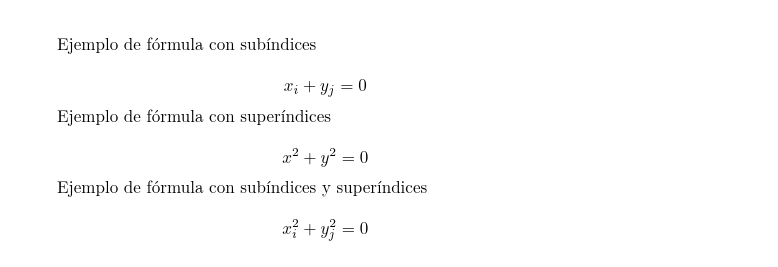
\includegraphics{./img/formulas/indices.png}
\end{tcolorbox}

Se pueden escribir subíndices de subíndices o superíndices de
superíndices anidando los comandos.

\hypertarget{fracciones}{%
\section{Fracciones}\label{fracciones}}

Para escribir fracciones simples en línea se puede usar el operador
aritmético \(/\) (por ejemplo \(3/4\)), pero para fracciones más
complejas o fracciones en modo display, conviene utilizar el comando
\texttt{\textbackslash{}frac\{num\}\{den\}}, donde \texttt{num} es el
numerador y \texttt{den} el denominador.

A su vez, se pueden escribir más fracciones en el numerador o el
denominador, anidando este comando.

\textbf{Ejemplo}

\begin{Shaded}
\begin{Highlighting}[]
\CommentTok{\% CUERPO}
\KeywordTok{\textbackslash{}begin}\NormalTok{\{}\ExtensionTok{document}\NormalTok{\}}
\NormalTok{Ejemplo de fracción en línea }\SpecialStringTok{$}\SpecialCharTok{\textbackslash{}frac}\SpecialStringTok{\{x+2\}\{x\^{}2{-}2x+1\}$}\NormalTok{.}

\NormalTok{Ejemplo de fracción en modo desplegado}

\SpecialStringTok{$$}
\SpecialCharTok{\textbackslash{}frac}\SpecialStringTok{\{}\SpecialCharTok{\textbackslash{}frac}\SpecialStringTok{\{x\}\{2\}+}\SpecialCharTok{\textbackslash{}frac}\SpecialStringTok{\{2\}\{3\}\}\{x\^{}2{-}2x+1\}}
\SpecialStringTok{$$}




\KeywordTok{\textbackslash{}end}\NormalTok{\{}\ExtensionTok{document}\NormalTok{\}}
\end{Highlighting}
\end{Shaded}

\begin{tcolorbox}[enhanced jigsaw, arc=.35mm, toprule=.15mm, opacitybacktitle=0.6, colback=white, coltitle=black, colbacktitle=quarto-callout-note-color!10!white, breakable, colframe=quarto-callout-note-color-frame, left=2mm, opacityback=0, bottomtitle=1mm, toptitle=1mm, titlerule=0mm, title={Salida}, bottomrule=.15mm, leftrule=.75mm, rightrule=.15mm]

\includegraphics{./img/formulas/fracciones.png}
\end{tcolorbox}

\hypertarget{sumatorios-productorios-e-integrales}{%
\section{Sumatorios, productorios e
integrales}\label{sumatorios-productorios-e-integrales}}

Para escribir sumatorios se utiliza el comando
\texttt{\textbackslash{}sum\_\{sub\}\^{}\{sup\}}, donde \(sub\) es el
subíndice que indica el inicio de la suma y \(sup\) es el superíndice
que indica el final de la suma. Si se quieren omitir los índices de
inicio y final de la suma, basta con el comando
\texttt{\textbackslash{}sum}.

De manera análoga, para escribir productorios se utiliza el comando
\texttt{\textbackslash{}prod\_\{sub\}\^{}\{sup\}}, donde \texttt{sub} es
el subíndice que indica el inicio del producto y \texttt{sup} es el
superíndice que indica el final del producto. Si se quieren omitir los
índices de inicio y final del producto, basta con el comando
\texttt{\textbackslash{}prod}.

\textbf{Ejemplo}

\begin{Shaded}
\begin{Highlighting}[]
\CommentTok{\% CUERPO}
\KeywordTok{\textbackslash{}begin}\NormalTok{\{}\ExtensionTok{document}\NormalTok{\}}
\NormalTok{Ejemplo de sumatorio}
\SpecialStringTok{$$}
\SpecialCharTok{\textbackslash{}sum}\SpecialStringTok{\_\{i=1\}\^{}\{}\SpecialCharTok{\textbackslash{}infty}\SpecialStringTok{\} x\^{}i}
\SpecialStringTok{$$}




\NormalTok{Ejemplo de productorio}
\SpecialStringTok{$$}
\SpecialCharTok{\textbackslash{}prod}\SpecialStringTok{\_\{i=1\}\^{}n i}
\SpecialStringTok{$$}



\KeywordTok{\textbackslash{}end}\NormalTok{\{}\ExtensionTok{document}\NormalTok{\}}
\end{Highlighting}
\end{Shaded}

\begin{tcolorbox}[enhanced jigsaw, arc=.35mm, toprule=.15mm, opacitybacktitle=0.6, colback=white, coltitle=black, colbacktitle=quarto-callout-note-color!10!white, breakable, colframe=quarto-callout-note-color-frame, left=2mm, opacityback=0, bottomtitle=1mm, toptitle=1mm, titlerule=0mm, title={Salida}, bottomrule=.15mm, leftrule=.75mm, rightrule=.15mm]
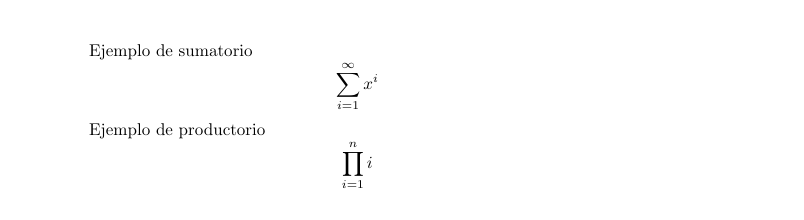
\includegraphics{./img/formulas/sumatorio.png}
\end{tcolorbox}

Del mismo modo, para escribir integrales definidas se utiliza el comando
\texttt{\textbackslash{}int\_\{sub\}\^{}\{sup\}}, donde \(sub\) es el
subíndice que indica el inicio de la integral y \(sup\) es el
superíndice que indica el final de la integral. Para integrales
indefinidas, basta con el comando \texttt{\textbackslash{}int}.

\textbf{Ejemplo}

\begin{Shaded}
\begin{Highlighting}[]
\CommentTok{\% CUERPO}
\KeywordTok{\textbackslash{}begin}\NormalTok{\{}\ExtensionTok{document}\NormalTok{\}}
\NormalTok{Ejemplo de integral definida}
\SpecialStringTok{$$}
\SpecialCharTok{\textbackslash{}int}\SpecialStringTok{\_a\^{}b f(x)}\SpecialCharTok{\textbackslash{},}\SpecialStringTok{dx}
\SpecialStringTok{$$}




\NormalTok{Ejemplo de integral indefinida}
\SpecialStringTok{$$}
\SpecialCharTok{\textbackslash{}int}\SpecialStringTok{ f(x)}\SpecialCharTok{\textbackslash{},}\SpecialStringTok{dx}
\SpecialStringTok{$$}



\KeywordTok{\textbackslash{}end}\NormalTok{\{}\ExtensionTok{document}\NormalTok{\}}
\end{Highlighting}
\end{Shaded}

\begin{tcolorbox}[enhanced jigsaw, arc=.35mm, toprule=.15mm, opacitybacktitle=0.6, colback=white, coltitle=black, colbacktitle=quarto-callout-note-color!10!white, breakable, colframe=quarto-callout-note-color-frame, left=2mm, opacityback=0, bottomtitle=1mm, toptitle=1mm, titlerule=0mm, title={Salida}, bottomrule=.15mm, leftrule=.75mm, rightrule=.15mm]
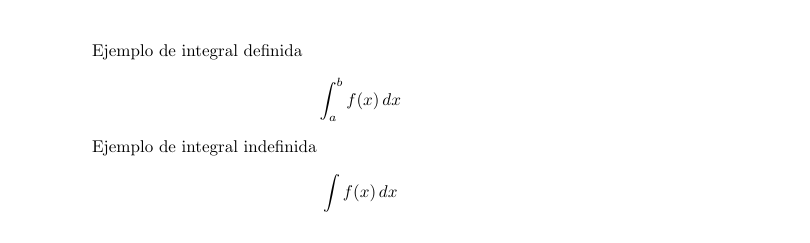
\includegraphics{./img/formulas/integral.png}
\end{tcolorbox}

\hypertarget{sombreros}{%
\section{Sombreros}\label{sombreros}}

Es posible poner símbolos encima de otros símbolos, más conocidos como
\emph{sombreros}. Los siguientes comandos sirven para poner distintos
tipos de sombreros:

\begin{itemize}
\tightlist
\item
  \texttt{\textbackslash{}bar\{...\}}: Linea horizontal para un
  carácter.
\item
  \texttt{\textbackslash{}overline\{...\}}: Línea horizontal para varios
  caracteres.
\item
  \texttt{\textbackslash{}hat}: Ángulo para un carácter.
\item
  \texttt{\textbackslash{}widehat}: Ángulo para varios caracteres.
\item
  \texttt{\textbackslash{}vec\{...\}}: Flecha para un carácter.
\item
  \texttt{\textbackslash{}overrightarrow\{...\}}: Flecha para varios
  caracteres.
\end{itemize}

\textbf{Ejemplo}

\begin{Shaded}
\begin{Highlighting}[]
\CommentTok{\% CUERPO}
\KeywordTok{\textbackslash{}begin}\NormalTok{\{}\ExtensionTok{document}\NormalTok{\}}
\NormalTok{Ejemplos de sombreros: }\SpecialStringTok{$}\SpecialCharTok{\textbackslash{}overline}\SpecialStringTok{\{xy\}$}\NormalTok{, }\SpecialStringTok{$}\SpecialCharTok{\textbackslash{}hat}\SpecialStringTok{\{a\}$}\NormalTok{, }\SpecialStringTok{$}\SpecialCharTok{\textbackslash{}widehat}\SpecialStringTok{\{abc\}$}\NormalTok{, }\SpecialStringTok{$}\SpecialCharTok{\textbackslash{}vec}\SpecialStringTok{\{u\}$}\NormalTok{.}
\KeywordTok{\textbackslash{}end}\NormalTok{\{}\ExtensionTok{document}\NormalTok{\}}
\end{Highlighting}
\end{Shaded}

\begin{tcolorbox}[enhanced jigsaw, arc=.35mm, toprule=.15mm, opacitybacktitle=0.6, colback=white, coltitle=black, colbacktitle=quarto-callout-note-color!10!white, breakable, colframe=quarto-callout-note-color-frame, left=2mm, opacityback=0, bottomtitle=1mm, toptitle=1mm, titlerule=0mm, title={Salida}, bottomrule=.15mm, leftrule=.75mm, rightrule=.15mm]

\includegraphics{./img/formulas/sombreros.png}
\end{tcolorbox}

\hypertarget{matrices}{%
\section{Matrices}\label{matrices}}

Las matrices se crean de manera similar a como se crean las tablas (ver
Capítulo~\ref{sec-tablas}), pero utilizando el entorno \texttt{array} en
lugar del entorno \texttt{tabular}. Para encerrar la matriz entre
paréntesis se pone el comando \texttt{\textbackslash{}left(} antes del
entorno y el comando \texttt{\textbackslash{}right)} después.

\textbf{Ejemplo}

\begin{Shaded}
\begin{Highlighting}[]
\CommentTok{\% CUERPO}
\KeywordTok{\textbackslash{}begin}\NormalTok{\{}\ExtensionTok{document}\NormalTok{\}}
\NormalTok{Ejemplo de matriz}
\SpecialStringTok{$$}
\SpecialCharTok{\textbackslash{}left}\SpecialStringTok{(}
\KeywordTok{\textbackslash{}begin}\NormalTok{\{}\ExtensionTok{array}\NormalTok{\}}\SpecialStringTok{\{rrr\}}
\SpecialStringTok{1 \& 2 \& 3 }\SpecialCharTok{\textbackslash{}\textbackslash{}}
\SpecialStringTok{x \& y \& z }\SpecialCharTok{\textbackslash{}\textbackslash{}}
\KeywordTok{\textbackslash{}end}\NormalTok{\{}\ExtensionTok{array}\NormalTok{\}}
\SpecialCharTok{\textbackslash{}right}\SpecialStringTok{)}
\SpecialStringTok{$$}



\KeywordTok{\textbackslash{}end}\NormalTok{\{}\ExtensionTok{document}\NormalTok{\}}
\end{Highlighting}
\end{Shaded}

\begin{tcolorbox}[enhanced jigsaw, arc=.35mm, toprule=.15mm, opacitybacktitle=0.6, colback=white, coltitle=black, colbacktitle=quarto-callout-note-color!10!white, breakable, colframe=quarto-callout-note-color-frame, left=2mm, opacityback=0, bottomtitle=1mm, toptitle=1mm, titlerule=0mm, title={Salida}, bottomrule=.15mm, leftrule=.75mm, rightrule=.15mm]

\includegraphics{./img/formulas/matriz.png}
\end{tcolorbox}

El paquete \texttt{amsmath} incorpora varios entornos más específicos
para matrices donde no es necesario especificar el número de columnas, y
tampoco los delimitadores:

\begin{itemize}
\tightlist
\item
  \texttt{matrix}: Matriz sin delimitadores (equivalente al entorno
  \texttt{array})
\item
  \texttt{pmatrix}: Matriz encerrada entre paréntesis.
\item
  \texttt{vmatrix}: Matriz encerrada entre barras verticales (por
  ejemplo para determinates).
\item
  \texttt{Vmatrix}: Matriz encerrada ente dobles barras verticales.
\item
  \texttt{bmatrix}: Matriz encerrada entre corchetes.
\item
  \texttt{Bmatrix}: Matriz encerrada entre llaves.
\end{itemize}

\textbf{Ejemplo}

\begin{Shaded}
\begin{Highlighting}[]
\CommentTok{\% PREÁMBULO}
\BuiltInTok{\textbackslash{}usepackage}\NormalTok{\{}\ExtensionTok{amsmath}\NormalTok{\}}
\CommentTok{\% CUERPO}
\KeywordTok{\textbackslash{}begin}\NormalTok{\{}\ExtensionTok{document}\NormalTok{\}}
\NormalTok{Ejemplo de determinante}

\SpecialStringTok{$$}
\KeywordTok{\textbackslash{}begin}\NormalTok{\{}\ExtensionTok{vmatrix}\NormalTok{\}}
\SpecialStringTok{1 \& x \& }\SpecialCharTok{\textbackslash{}alpha}\SpecialStringTok{ }\SpecialCharTok{\textbackslash{}\textbackslash{}}
\SpecialStringTok{2 \& y \& }\SpecialCharTok{\textbackslash{}beta}\SpecialStringTok{ }\SpecialCharTok{\textbackslash{}\textbackslash{}}
\SpecialStringTok{3 \& z \&}\SpecialCharTok{\textbackslash{}gamma}
\KeywordTok{\textbackslash{}end}\NormalTok{\{}\ExtensionTok{vmatrix}\NormalTok{\}}
\SpecialStringTok{$$}



\KeywordTok{\textbackslash{}end}\NormalTok{\{}\ExtensionTok{document}\NormalTok{\}}
\end{Highlighting}
\end{Shaded}

\begin{tcolorbox}[enhanced jigsaw, arc=.35mm, toprule=.15mm, opacitybacktitle=0.6, colback=white, coltitle=black, colbacktitle=quarto-callout-note-color!10!white, breakable, colframe=quarto-callout-note-color-frame, left=2mm, opacityback=0, bottomtitle=1mm, toptitle=1mm, titlerule=0mm, title={Salida}, bottomrule=.15mm, leftrule=.75mm, rightrule=.15mm]

\includegraphics{./img/formulas/determinante.png}
\end{tcolorbox}

\hypertarget{teoremas}{%
\section{Teoremas}\label{teoremas}}

Para crear denificiones, teoremas, proposiciones, corolarios y otros
tipos de enunciados de sebe cargar el paquete \texttt{amsthm} y definir
los tipos de enunciados en el preámbulo con el comando
\texttt{\textbackslash{}newtheorem\{entorno\}\{texo\}}, donde
\texttt{entorno} es el nombre del entorno y \texttt{texto} el texto que
aparerá en el documento final como encabezado del enunciado.

Estos entornos admiten como argumento opcional un texto que se utiliza
para dar nombre al enunciado.

Los enunciados definidos con este comando aparecen por defecto numerados
para poder referenciarlos en otras partes del documento, pero se pueden
definir entornos no numerados con la variante del comando anterior
\texttt{\textbackslash{}newtheorem*\{entorno\}\{texo\}}

Para demostraciones se puede utilizar el entorno \texttt{proof}.

\textbf{Ejemplo}

\begin{Shaded}
\begin{Highlighting}[]
\CommentTok{\% PREÁMBULO}
\BuiltInTok{\textbackslash{}usepackage}\NormalTok{\{}\ExtensionTok{amsmath}\NormalTok{\}}
\FunctionTok{\textbackslash{}DeclareMathOperator}\NormalTok{\{}\FunctionTok{\textbackslash{}sen}\NormalTok{\}\{sen\}}
\BuiltInTok{\textbackslash{}usepackage}\NormalTok{\{}\ExtensionTok{amsthm}\NormalTok{\}}
\FunctionTok{\textbackslash{}newtheorem}\NormalTok{\{midef\}\{Definición\}}
\FunctionTok{\textbackslash{}newtheorem}\NormalTok{\{teo\}\{Teorema\}}

\CommentTok{\% CUERPO}
\KeywordTok{\textbackslash{}begin}\NormalTok{\{}\ExtensionTok{document}\NormalTok{\}}

\KeywordTok{\textbackslash{}begin}\NormalTok{\{}\ExtensionTok{midef}\NormalTok{\}}
\NormalTok{Dado un triángulo rectángulo de catetos }\SpecialStringTok{$a$}\NormalTok{, }\SpecialStringTok{$b$}\NormalTok{ e hipotenusa }\SpecialStringTok{$c$}\NormalTok{, se define}
\NormalTok{el seno del ángulo }\SpecialStringTok{$}\SpecialCharTok{\textbackslash{}alpha}\SpecialStringTok{$}\NormalTok{ opuesto al cateto }\SpecialStringTok{$b$}\NormalTok{ como }

\SpecialStringTok{$$}
\SpecialCharTok{\textbackslash{}sen}\SpecialStringTok{\{}\SpecialCharTok{\textbackslash{}alpha}\SpecialStringTok{\}= }\SpecialCharTok{\textbackslash{}frac}\SpecialStringTok{\{b\}\{c\}.}
\SpecialStringTok{$$}



\KeywordTok{\textbackslash{}end}\NormalTok{\{}\ExtensionTok{midef}\NormalTok{\}}

\KeywordTok{\textbackslash{}begin}\NormalTok{\{}\ExtensionTok{teo}\NormalTok{\}}
\NormalTok{Para cualquier ángulo }\SpecialStringTok{$}\SpecialCharTok{\textbackslash{}alpha}\SpecialStringTok{$}\NormalTok{ se cumple }
\SpecialStringTok{$}\SpecialCharTok{\textbackslash{}sen}\SpecialStringTok{(}\SpecialCharTok{\textbackslash{}alpha}\SpecialStringTok{)\^{}2 + }\SpecialCharTok{\textbackslash{}cos}\SpecialStringTok{(}\SpecialCharTok{\textbackslash{}alpha}\SpecialStringTok{)\^{}2 = 1$}\NormalTok{.}
\KeywordTok{\textbackslash{}end}\NormalTok{\{}\ExtensionTok{teo}\NormalTok{\}}

\KeywordTok{\textbackslash{}begin}\NormalTok{\{}\ExtensionTok{proof}\NormalTok{\}}
\NormalTok{Es una consecuencia directa del teorema de Pitágoras.}
\KeywordTok{\textbackslash{}end}\NormalTok{\{}\ExtensionTok{proof}\NormalTok{\}}
\KeywordTok{\textbackslash{}end}\NormalTok{\{}\ExtensionTok{document}\NormalTok{\}}
\end{Highlighting}
\end{Shaded}

\begin{tcolorbox}[enhanced jigsaw, arc=.35mm, toprule=.15mm, opacitybacktitle=0.6, colback=white, coltitle=black, colbacktitle=quarto-callout-note-color!10!white, breakable, colframe=quarto-callout-note-color-frame, left=2mm, opacityback=0, bottomtitle=1mm, toptitle=1mm, titlerule=0mm, title={Salida}, bottomrule=.15mm, leftrule=.75mm, rightrule=.15mm]
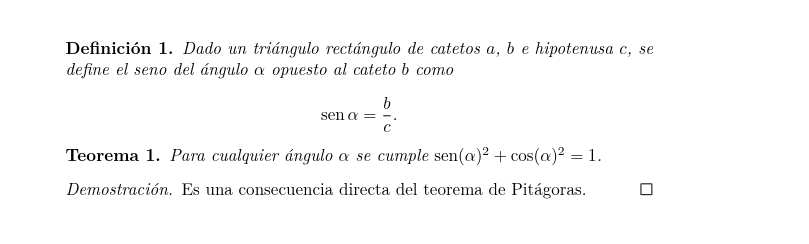
\includegraphics{./img/formulas/teoremas.png}
\end{tcolorbox}

\begin{tcolorbox}[enhanced jigsaw, arc=.35mm, toprule=.15mm, opacitybacktitle=0.6, colback=white, coltitle=black, colbacktitle=quarto-callout-tip-color!10!white, breakable, colframe=quarto-callout-tip-color-frame, left=2mm, opacityback=0, bottomtitle=1mm, toptitle=1mm, titlerule=0mm, title=\textcolor{quarto-callout-tip-color}{\faLightbulb}\hspace{0.5em}{Tip}, bottomrule=.15mm, leftrule=.75mm, rightrule=.15mm]
Se recomienda cargar los paquetes \texttt{amsmath}, \texttt{amssymb} y
\texttt{amsthm} para documentos extensos o con muchas fórmulas
matemáticas.
\end{tcolorbox}

\bookmarksetup{startatroot}

\hypertarget{entornos-flotantes}{%
\chapter{Entornos flotantes}\label{entornos-flotantes}}

Hay determinados contenidos, como por ejemplo las tablas o las imágenes
que son bloques indivisibles, de manera que cuando no hay espacio
suficiente en la página para encajarlos, pasan a colocarse en la
siguiente página, dejando en la página anterior un espacio vertical
vacío poco estético.

La solución consiste en incluir estos contenidos en un entorno flotante,
que se ubicará automáticamente sin dejar espacios vacíos. Como estos
contenidos pueden aparecer lejos de su posición en el código fuente,
para que no estén descontextualizados suelen llevar asociada una
leyenda.

Existen dos entornos flotantes, para figuras y tablas.

\hypertarget{entorno-flotante-para-figuras}{%
\section{Entorno flotante para
figuras}\label{entorno-flotante-para-figuras}}

El entorno flotante para figuras es \texttt{figure} tiene el siguiente
esqueleto.

\begin{Shaded}
\begin{Highlighting}[]
\KeywordTok{\textbackslash{}begin}\NormalTok{\{}\ExtensionTok{figure}\NormalTok{\}[posición]}
\NormalTok{    Código de las imágenes}
\KeywordTok{\textbackslash{}label}\NormalTok{\{}\ExtensionTok{etiqueta}\NormalTok{\}}
\FunctionTok{\textbackslash{}caption}\NormalTok{\{leyenda\}}
\KeywordTok{\textbackslash{}end}\NormalTok{\{}\ExtensionTok{figure}\NormalTok{\}}
\end{Highlighting}
\end{Shaded}

El argumento opcional indica la preferencia de ubicación de la figura en
la página (\texttt{h} en el lugar en el que aparece en el código fuente,
\texttt{t} arriba, \texttt{b} abajo). \LaTeX intentará ubicar la
figura en esa posición salvo que no sea posible.

Las figuras flotantes se numeran automáticamente y el comando
\texttt{\textbackslash{}label\{...\}} asigna una etiqueta al entorno
flotante para poder referenciarlo desde otras partes del documento. Por
su parte, el comando \texttt{\textbackslash{}caption\{...\}} crea la
leyenda de la figura.

\begin{Shaded}
\begin{Highlighting}[]
\CommentTok{\% PREÁMBULO}
\BuiltInTok{\textbackslash{}usepackage}\NormalTok{\{}\ExtensionTok{graphicx}\NormalTok{\}}
\CommentTok{\% CUERPO}
\KeywordTok{\textbackslash{}begin}\NormalTok{\{}\ExtensionTok{document}\NormalTok{\}}
\NormalTok{Ejemplo de imagen flotante. Como se puede apreciar la imagen aparece al }
\NormalTok{principio de la página aunque va después de este párrafo en el código }
\NormalTok{fuente.}

\KeywordTok{\textbackslash{}begin}\NormalTok{\{}\ExtensionTok{figure}\NormalTok{\}[t]}
\KeywordTok{\textbackslash{}begin}\NormalTok{\{}\ExtensionTok{center}\NormalTok{\}}
\BuiltInTok{\textbackslash{}includegraphics}\NormalTok{\{}\ExtensionTok{img/logo{-}aprendeconalf.png}\NormalTok{\}}
\KeywordTok{\textbackslash{}end}\NormalTok{\{}\ExtensionTok{center}\NormalTok{\}}
\KeywordTok{\textbackslash{}label}\NormalTok{\{}\ExtensionTok{img{-}1}\NormalTok{\}}
\FunctionTok{\textbackslash{}caption}\NormalTok{\{Logotipo del sitio web AprendeconAlf.\}}
\KeywordTok{\textbackslash{}end}\NormalTok{\{}\ExtensionTok{figure}\NormalTok{\}}
\KeywordTok{\textbackslash{}end}\NormalTok{\{}\ExtensionTok{document}\NormalTok{\}}
\end{Highlighting}
\end{Shaded}

\begin{tcolorbox}[enhanced jigsaw, arc=.35mm, toprule=.15mm, opacitybacktitle=0.6, colback=white, coltitle=black, colbacktitle=quarto-callout-note-color!10!white, breakable, colframe=quarto-callout-note-color-frame, left=2mm, opacityback=0, bottomtitle=1mm, toptitle=1mm, titlerule=0mm, title={Salida}, bottomrule=.15mm, leftrule=.75mm, rightrule=.15mm]
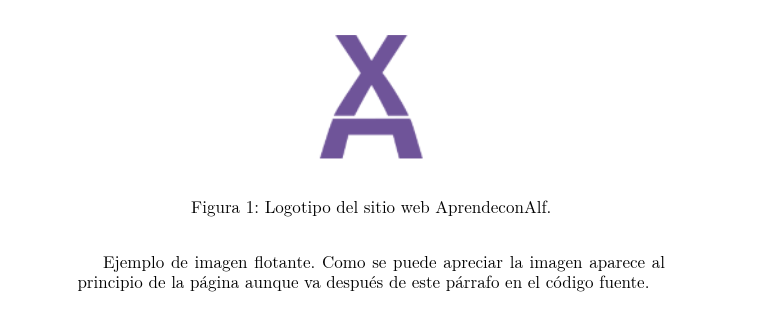
\includegraphics{./img/entornos-flotantes/figura-flotante.png}
\end{tcolorbox}

Para incluir el listado de figuras de un documento en cualquier parte se
utiliza el comando \texttt{\textbackslash{}listoffigures}.

\hypertarget{entorno-flotante-para-tablas}{%
\section{Entorno flotante para
tablas}\label{entorno-flotante-para-tablas}}

El entorno flotante para tablas es \texttt{table} y su esqueleto es muy
parecido al del entorno para figuras.

\begin{Shaded}
\begin{Highlighting}[]
\KeywordTok{\textbackslash{}begin}\NormalTok{\{}\ExtensionTok{table}\NormalTok{\}[posición]}
\NormalTok{    Código de la tabla}
\KeywordTok{\textbackslash{}label}\NormalTok{\{}\ExtensionTok{etiqueta}\NormalTok{\}}
\FunctionTok{\textbackslash{}caption}\NormalTok{\{leyenda\}}
\KeywordTok{\textbackslash{}end}\NormalTok{\{}\ExtensionTok{table}\NormalTok{\}}
\end{Highlighting}
\end{Shaded}

Las tablas, al igual que las figuras, se enumeran automáticamente y
pueden referenciarse después asignándoles una etiqueta con el comando
\texttt{\textbackslash{}label\{...\}}.

\begin{Shaded}
\begin{Highlighting}[]
\CommentTok{\% CUERPO}
\KeywordTok{\textbackslash{}begin}\NormalTok{\{}\ExtensionTok{document}\NormalTok{\}}
\NormalTok{Ejemplo de tabla flotante. Como se puede apreciar la tabla aparece al }
\NormalTok{principio de la página aunque va después de este párrafo en el código }
\NormalTok{fuente.}

\KeywordTok{\textbackslash{}begin}\NormalTok{\{}\ExtensionTok{table}\NormalTok{\}[t]}
\KeywordTok{\textbackslash{}begin}\NormalTok{\{}\ExtensionTok{center}\NormalTok{\}}
\KeywordTok{\textbackslash{}begin}\NormalTok{\{}\ExtensionTok{tabular}\NormalTok{\}\{|l|c|r|\}}
\FunctionTok{\textbackslash{}hline}
\NormalTok{Nombre }\OperatorTok{\&}\NormalTok{ Ciudad }\OperatorTok{\&}\NormalTok{ Edad }\FunctionTok{\textbackslash{}\textbackslash{}} 
\FunctionTok{\textbackslash{}hline}
\FunctionTok{\textbackslash{}hline}
\NormalTok{María }\OperatorTok{\&}\NormalTok{ Valencia }\OperatorTok{\&}\NormalTok{ 22 }\FunctionTok{\textbackslash{}\textbackslash{}}
\FunctionTok{\textbackslash{}hline}
\NormalTok{Juan }\OperatorTok{\&}\NormalTok{ Madrid }\OperatorTok{\&}\NormalTok{ 50 }\FunctionTok{\textbackslash{}\textbackslash{}}
\FunctionTok{\textbackslash{}hline}
\NormalTok{Carmen }\OperatorTok{\&}\NormalTok{ Barcelona }\OperatorTok{\&}\NormalTok{ 35 }\FunctionTok{\textbackslash{}\textbackslash{}}
\FunctionTok{\textbackslash{}hline}
\KeywordTok{\textbackslash{}end}\NormalTok{\{}\ExtensionTok{tabular}\NormalTok{\}}
\KeywordTok{\textbackslash{}end}\NormalTok{\{}\ExtensionTok{center}\NormalTok{\}}
\KeywordTok{\textbackslash{}label}\NormalTok{\{}\ExtensionTok{img{-}1}\NormalTok{\}}
\FunctionTok{\textbackslash{}caption}\NormalTok{\{Tabla de clientes de una empresa.\}}
\KeywordTok{\textbackslash{}end}\NormalTok{\{}\ExtensionTok{table}\NormalTok{\}}
\KeywordTok{\textbackslash{}end}\NormalTok{\{}\ExtensionTok{document}\NormalTok{\}}
\end{Highlighting}
\end{Shaded}

\begin{tcolorbox}[enhanced jigsaw, arc=.35mm, toprule=.15mm, opacitybacktitle=0.6, colback=white, coltitle=black, colbacktitle=quarto-callout-note-color!10!white, breakable, colframe=quarto-callout-note-color-frame, left=2mm, opacityback=0, bottomtitle=1mm, toptitle=1mm, titlerule=0mm, title={Salida}, bottomrule=.15mm, leftrule=.75mm, rightrule=.15mm]
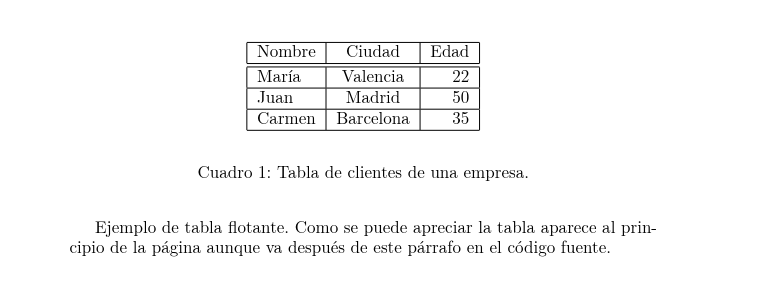
\includegraphics{./img/entornos-flotantes/tabla-flotante.png}
\end{tcolorbox}

Para incluir el listado de figuras de un documento en cualquier parte se
utiliza el comando \texttt{\textbackslash{}listoftables}.

\bookmarksetup{startatroot}

\hypertarget{referencias-cruzadas-y-notas-a-pie}{%
\chapter{Referencias cruzadas y notas a
pie}\label{referencias-cruzadas-y-notas-a-pie}}

Otro de los puntos fuertes de \LaTeX es la gestión de las
referencias cruzadas, es decir, referencias a otras partes del
documento, así como las notas a pie de página.

\hypertarget{referencias-cruzadas}{%
\section{Referencias cruzadas}\label{referencias-cruzadas}}

Como se ha visto, muchos elementos de un documento están enumerados:
capítulos, secciones, figuras, tablas, ecuaciones, teoremas, páginas,
etc. Para poder referenciarlos, cada elemento debe tener asignada una
etiqueta única. Para asignar una etiqueta a cualquier elemento numerado
se utiliza el comando \texttt{\textbackslash{}label\{etiqueta\}}. Este
comando debe ubicarse justo antes o después del elemento que quiere
etiquetar.

Posteriormente, para hacer una referencia al elemento en otra parte del
documento se utiliza el comando
\texttt{\textbackslash{}ref\{etiqueta\}}.

\textbf{Ejemplo}

\begin{Shaded}
\begin{Highlighting}[]
\CommentTok{\% PREÁMBULO}
\BuiltInTok{\textbackslash{}usepackage}\NormalTok{\{}\ExtensionTok{amsmath}\NormalTok{\}}
\FunctionTok{\textbackslash{}DeclareMathOperator}\NormalTok{\{}\FunctionTok{\textbackslash{}sen}\NormalTok{\}\{sen\}}
\BuiltInTok{\textbackslash{}usepackage}\NormalTok{\{}\ExtensionTok{amsthm}\NormalTok{\}}
\FunctionTok{\textbackslash{}newtheorem}\NormalTok{\{teo\}\{Teorema\}}

\CommentTok{\% CUERPO}
\KeywordTok{\textbackslash{}begin}\NormalTok{\{}\ExtensionTok{document}\NormalTok{\}}
\KeywordTok{\textbackslash{}begin}\NormalTok{\{}\ExtensionTok{teo}\NormalTok{\}}\KeywordTok{\textbackslash{}label}\NormalTok{\{}\ExtensionTok{teo{-}trigo}\NormalTok{\}}
\NormalTok{Para cualquier ángulo}
\SpecialStringTok{$}\SpecialCharTok{\textbackslash{}alpha}\SpecialStringTok{$}\NormalTok{ se cumple }
\KeywordTok{\textbackslash{}begin}\NormalTok{\{}\ExtensionTok{equation}\NormalTok{\}}\SpecialCharTok{\textbackslash{}label}\SpecialStringTok{\{eq{-}trigo\}}
\SpecialCharTok{\textbackslash{}sen}\SpecialStringTok{(}\SpecialCharTok{\textbackslash{}alpha}\SpecialStringTok{)\^{}2 + }\SpecialCharTok{\textbackslash{}cos}\SpecialStringTok{(}\SpecialCharTok{\textbackslash{}alpha}\SpecialStringTok{)\^{}2 = 1.}
\KeywordTok{\textbackslash{}end}\NormalTok{\{}\ExtensionTok{equation}\NormalTok{\}}
\KeywordTok{\textbackslash{}end}\NormalTok{\{}\ExtensionTok{teo}\NormalTok{\}}

\NormalTok{Ejemplo de referencia cruzada. La ecuación }\KeywordTok{\textbackslash{}ref}\NormalTok{\{}\ExtensionTok{eq{-}trigo}\NormalTok{\} del teorema }
\KeywordTok{\textbackslash{}ref}\NormalTok{\{}\ExtensionTok{teo{-}trigo}\NormalTok{\} es una ecuación básica en trigonometría.}
\KeywordTok{\textbackslash{}end}\NormalTok{\{}\ExtensionTok{document}\NormalTok{\}}
\end{Highlighting}
\end{Shaded}

\begin{tcolorbox}[enhanced jigsaw, arc=.35mm, toprule=.15mm, opacitybacktitle=0.6, colback=white, coltitle=black, colbacktitle=quarto-callout-note-color!10!white, breakable, colframe=quarto-callout-note-color-frame, left=2mm, opacityback=0, bottomtitle=1mm, toptitle=1mm, titlerule=0mm, title={Salida}, bottomrule=.15mm, leftrule=.75mm, rightrule=.15mm]
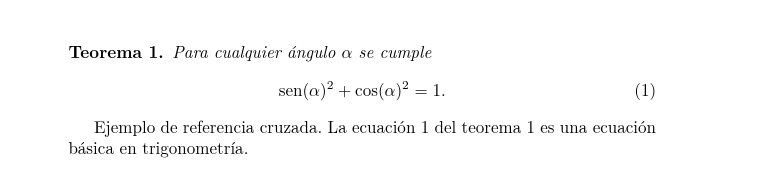
\includegraphics{./img/referencias-cruzadas/referencias-cruzadas.png}
\end{tcolorbox}

\hypertarget{notas-a-pie-de-puxe1gina}{%
\section{Notas a pie de página}\label{notas-a-pie-de-puxe1gina}}

Para insertar una nota a pié de página se utiliza el comando
\texttt{\textbackslash{}footnote\{...\}}.

\textbf{Ejemplo}

\begin{Shaded}
\begin{Highlighting}[]
\CommentTok{\% CUERPO}
\KeywordTok{\textbackslash{}begin}\NormalTok{\{}\ExtensionTok{document}\NormalTok{\}}
\NormalTok{El logotipo de latex es }\SpecialStringTok{$}\SpecialCharTok{\textbackslash{}LaTeX}\SpecialStringTok{$}\NormalTok{.}\FunctionTok{\textbackslash{}footnote}\NormalTok{\{Fue creado por Leslie Lamport.\}}
\KeywordTok{\textbackslash{}end}\NormalTok{\{}\ExtensionTok{document}\NormalTok{\}}
\end{Highlighting}
\end{Shaded}

\begin{tcolorbox}[enhanced jigsaw, arc=.35mm, toprule=.15mm, opacitybacktitle=0.6, colback=white, coltitle=black, colbacktitle=quarto-callout-note-color!10!white, breakable, colframe=quarto-callout-note-color-frame, left=2mm, opacityback=0, bottomtitle=1mm, toptitle=1mm, titlerule=0mm, title={Salida}, bottomrule=.15mm, leftrule=.75mm, rightrule=.15mm]
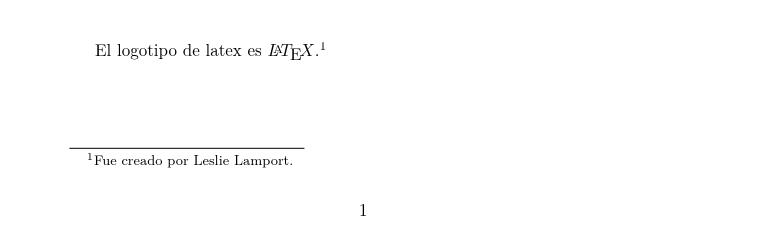
\includegraphics{./img/referencias-cruzadas/nota-pie.png}
\end{tcolorbox}

\bookmarksetup{startatroot}

\hypertarget{citas-y-referencias-bibliogruxe1ficas}{%
\chapter{Citas y referencias
bibliográficas}\label{citas-y-referencias-bibliogruxe1ficas}}

Al igual que con las referencias cruzadas, \LaTeX hace un
maravilloso trabajo con las citas de referencias bibliográficas. Para
ello se apoya en otro programa de gestión de referencias bibliográficas
llamado \href{http://www.bibtex.org/}{BibTeX}, que viene incluido en la
distribución estándar de \LaTeX. BibTeX permite crear una base de
datos de distintos tipos de documentos que después se pueden citar en
nuestro documento y después listar al final del documento las
referencias bibliográficas citadas con diferentes formatos.

También existe otro gestor de referencias bibliográficas llamado
\texttt{biber} que soporta la codificación de caracteres unicode, y por
tanto es más apropiado si vamos a compilar nuestro documento con
\texttt{xelatex}.

Para incluir referencias bibliográficas en un documento primero hay que
crear una base de datos con las fuentes bibliográficas que vayamos a
usar en un documento. Esa base de datos se crea en un fichero de texto
independiente con el formato que requiere BibTex con extensión
\texttt{.bib}.

La sintaxis para crear una nueva entrada bibliográfica en la base de
datos es un poco compleja al principio, pero afortunadamente existen
bastantes aplicaciones de gestión bibliográfica, como
\href{https://www.zotero.org/}{Zotero},
\href{https://www.mendeley.com/}{Mendely},
\href{https://endnote.com/}{EndNote} o
\href{https://refworks.proquest.com/researcher/}{RefWorks} o
\href{https://www.bibsonomy.org/}{BibSonomy} que incluyen la posibilidad
de exportar la bibliografía en ese formato.

\textbf{Ejemplo}

El siguiente fichero contiene una base de datos bibliográfica con dos
entradas, un libro y un artículo de una revista.

\begin{Shaded}
\begin{Highlighting}[]
\CommentTok{\% Fichero bibliografia.tex}
\NormalTok{@book\{lamport\_latex\_1994,}
\NormalTok{    edition = \{2nd\},}
\NormalTok{    title = \{\{LaTeX\}: \{A\} \{Document\} \{Preparation\} \{System\}, 2nd \{Edition\}\},}
\NormalTok{    isbn = \{978{-}0{-}201{-}52983{-}8\},}
\NormalTok{    publisher = \{Addison{-}Wesley Professional.\},}
\NormalTok{    author = \{Lamport, Leslie\},}
\NormalTok{    month = jun,}
\NormalTok{    year = \{1994\}}
\NormalTok{\}}

\NormalTok{@article\{borbon\_latex\_2022,}
\NormalTok{    title = \{\{LaTeX\}: \{Primeros\} pasos\},}
\NormalTok{    journal = \{Revista digital Matemática, Educación e Internet.\},}
\NormalTok{    author = \{\{Borbón, Alexánder\} and \{Mora, Walter\}\},}
\NormalTok{    year = \{2022\},}
\NormalTok{    pages = \{2{-}{-}7\},}
\NormalTok{\}}
\end{Highlighting}
\end{Shaded}

Obsérvese que cada entrada bibliográfica empieza por el tipo de
documento (book, article, etc.) y está descrita por varios campos: title
(título), author (autor), journal (revista), year (año), etc. El primer
campo es una clave que identifica al documento de manera única y que se
utilizará posteriormente para citarlo.

Una vez creada la base de datos, para citar cualquier referencia
contenida en ella, hay que cargar en el preámbulo el paquete
\texttt{biblatex} e indicar la ubicación de la base de datos con el
comando \texttt{addbibresource\{bibliografia.bib\}}, donde
\texttt{bibliografia.bib} es el nombre del fichero con la base de datos
bibliográfica (incluida la ruta), y luego escribir el comando
\texttt{\textbackslash{}cite\{clave\}}, donde \texttt{clave} es la clave
de la entrada bibliográfica en la base de datos, en el lugar donde se
quiera hacer la referencia.

Finalmente para listar las referencias bibliográficas citadas en el
documento basta con insertar el comando
\texttt{\textbackslash{}printbibliography}.

\textbf{Ejemplo}

\begin{Shaded}
\begin{Highlighting}[]
\CommentTok{\% PREÁMBULO}
\BuiltInTok{\textbackslash{}usepackage}\NormalTok{\{}\ExtensionTok{biblatex}\NormalTok{\}}
\FunctionTok{\textbackslash{}addbibresource}\NormalTok{\{bibliografia.bib\}}
\CommentTok{\% CUERPO}
\KeywordTok{\textbackslash{}begin}\NormalTok{\{}\ExtensionTok{document}\NormalTok{\}}
\NormalTok{El principal libro sobre latex es }\KeywordTok{\textbackslash{}cite}\NormalTok{\{}\ExtensionTok{lamport\_latex\_1994}\NormalTok{\}, aunque también }
\NormalTok{es muy interesante el artículo }\KeywordTok{\textbackslash{}cite}\NormalTok{\{}\ExtensionTok{borbon\_latex\_2022}\NormalTok{\}}

\FunctionTok{\textbackslash{}printbibliography}
\KeywordTok{\textbackslash{}end}\NormalTok{\{}\ExtensionTok{document}\NormalTok{\}}
\end{Highlighting}
\end{Shaded}

\begin{tcolorbox}[enhanced jigsaw, arc=.35mm, toprule=.15mm, opacitybacktitle=0.6, colback=white, coltitle=black, colbacktitle=quarto-callout-note-color!10!white, breakable, colframe=quarto-callout-note-color-frame, left=2mm, opacityback=0, bottomtitle=1mm, toptitle=1mm, titlerule=0mm, title={Salida}, bottomrule=.15mm, leftrule=.75mm, rightrule=.15mm]
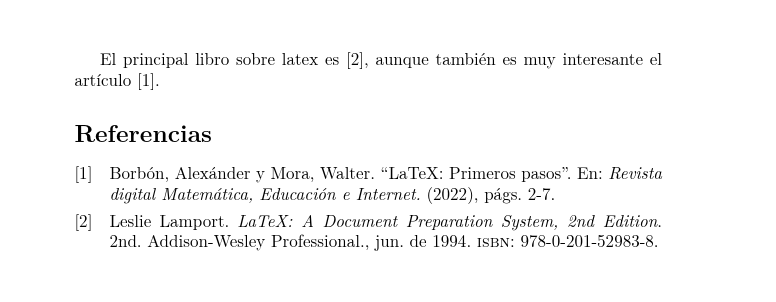
\includegraphics{./img/bibliografia/bibliografia.png}
\end{tcolorbox}

Existen diferentes estilos para las citaciones y para el listado con las
referencias bibliográficas que se pueden indicar en la carga del paquete
\texttt{biblatex} con el parámetro opcional \texttt{style}. Por ejemplo
si en lugar de números en las citaciones queremos que aparezca las
iniciales del autor y el año, hay que seleccionar el estilo
\texttt{style=alphabetic}. En el siguiente enlace existe un listado
exahustivo de los diferentes
\href{https://www.overleaf.com/learn/latex/Biblatex_citation_styles}{estilos
de citación}.

Por último si en lugar de \texttt{bibtex} se quiere usar \texttt{biber}
para gestionar las referencias bibliográficas, hay que indicarlo también
ebn la carga del paquete \texttt{biblatex} mediante el parámetro
opcional \texttt{backend=biber}.

\textbf{Ejemplo}

\begin{Shaded}
\begin{Highlighting}[]
\CommentTok{\% PREÁMBULO}
\BuiltInTok{\textbackslash{}usepackage}\NormalTok{[}
\NormalTok{backend=biber, style=alphabetic]\{}\ExtensionTok{biblatex}\NormalTok{\}}
\FunctionTok{\textbackslash{}addbibresource}\NormalTok{\{bibliografia.bib\}}
\CommentTok{\% CUERPO}
\KeywordTok{\textbackslash{}begin}\NormalTok{\{}\ExtensionTok{document}\NormalTok{\}}
\NormalTok{El principal libro sobre latex es }\KeywordTok{\textbackslash{}cite}\NormalTok{\{}\ExtensionTok{lamport\_latex\_1994}\NormalTok{\}, aunque también }
\NormalTok{es muy interesante el artículo }\KeywordTok{\textbackslash{}cite}\NormalTok{\{}\ExtensionTok{borbon\_latex\_2022}\NormalTok{\}}

\FunctionTok{\textbackslash{}printbibliography}
\KeywordTok{\textbackslash{}end}\NormalTok{\{}\ExtensionTok{document}\NormalTok{\}}
\end{Highlighting}
\end{Shaded}

\begin{tcolorbox}[enhanced jigsaw, arc=.35mm, toprule=.15mm, opacitybacktitle=0.6, colback=white, coltitle=black, colbacktitle=quarto-callout-note-color!10!white, breakable, colframe=quarto-callout-note-color-frame, left=2mm, opacityback=0, bottomtitle=1mm, toptitle=1mm, titlerule=0mm, title={Salida}, bottomrule=.15mm, leftrule=.75mm, rightrule=.15mm]
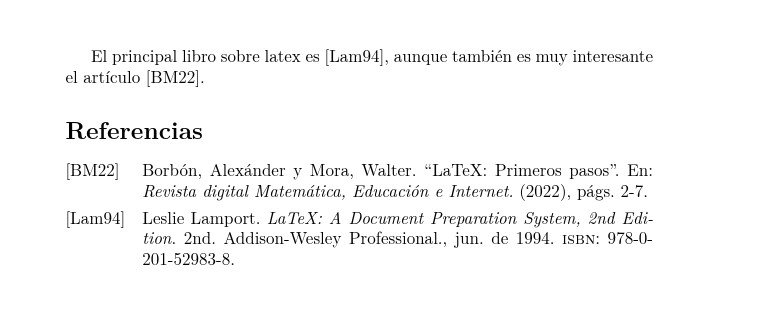
\includegraphics{./img/bibliografia/bibliografia2.png}
\end{tcolorbox}

\bookmarksetup{startatroot}

\hypertarget{diseuxf1o-de-puxe1gina}{%
\chapter{Diseño de página}\label{diseuxf1o-de-puxe1gina}}

Existen distintos parámetros que determinan el aspecto final de una
página con texto. En este capítulo veremos como modificar las
dimensiones de la página, los márgenes, y cómo introducir encabezados y
pies.

\hypertarget{dimensiones-y-muxe1rgenes}{%
\section{Dimensiones y márgenes}\label{dimensiones-y-muxe1rgenes}}

Aunque es posible definir el tamaño de la página como un argumento del
comando que define la clase del documento
\texttt{\textbackslash{}documentclass}, si queremos tener mayor control
sobre las dimensiones del documento, así como de los márgenes, conviene
utilizar el paquete \texttt{geometry}.

El paquete \texttt{geometry} permite definir las dimensiones de la
página mediante un argumento opcional con distintos tamaños de página
predefinidos (\texttt{a4paper}, \texttt{a5paper}, \texttt{b1paper},
\texttt{letterpaper}, etc.), pero también es posible definir nuestras
propias dimensiones con los siguientes argumentos:

\begin{itemize}
\tightlist
\item
  \texttt{paperheight=x} establece la longitud vertical de la página en
  \texttt{x} (es necesario indicar las unidades \texttt{pt},\texttt{mm}
  o \texttt{cm})
\item
  \texttt{paperwidth=x} establece la longitud horizontal de la página en
  \texttt{x}.
\end{itemize}

Por defecto la orientación del documento es vertical, pero puede ponerse
en formato horizontal o apaisado con el argumento \texttt{landscape}.

\textbf{Ejemplo}

\begin{Shaded}
\begin{Highlighting}[]
\CommentTok{\% PREÁMBULO}
\BuiltInTok{\textbackslash{}usepackage}\NormalTok{[a5paper, landscape]\{}\ExtensionTok{geometry}\NormalTok{\}}
\BuiltInTok{\textbackslash{}usepackage}\NormalTok{\{}\ExtensionTok{blindtext}\NormalTok{\}}

\CommentTok{\% CUERPO}
\KeywordTok{\textbackslash{}begin}\NormalTok{\{}\ExtensionTok{document}\NormalTok{\}}
\KeywordTok{\textbackslash{}section}\NormalTok{\{Introducción\}}
\NormalTok{Esta es una página de tamaño A5 apaisada.}

\KeywordTok{\textbackslash{}subsection}\NormalTok{\{Texto de relleno\}}
\FunctionTok{\textbackslash{}blindtext}\NormalTok{[2]}

\KeywordTok{\textbackslash{}end}\NormalTok{\{}\ExtensionTok{document}\NormalTok{\}}
\end{Highlighting}
\end{Shaded}

\begin{tcolorbox}[enhanced jigsaw, arc=.35mm, toprule=.15mm, opacitybacktitle=0.6, colback=white, coltitle=black, colbacktitle=quarto-callout-note-color!10!white, breakable, colframe=quarto-callout-note-color-frame, left=2mm, opacityback=0, bottomtitle=1mm, toptitle=1mm, titlerule=0mm, title={Salida}, bottomrule=.15mm, leftrule=.75mm, rightrule=.15mm]
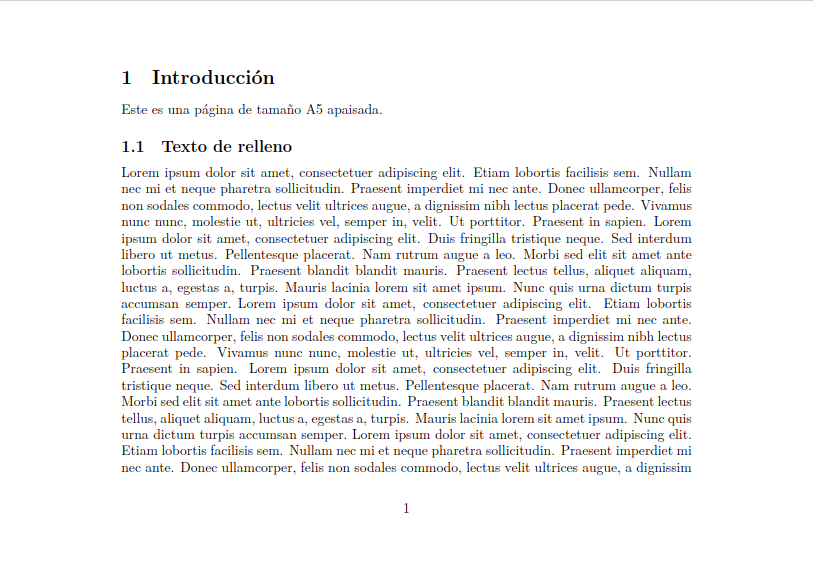
\includegraphics{./img/diseño-pagina/pagina-a5-apaisada.png}
\end{tcolorbox}

También permite definir los márgenes del documento mediante los
siguientes argumentos:

\begin{itemize}
\tightlist
\item
  \texttt{margin=x} establece los cuatro márgenes (izquierdo, derecho,
  superior e inferior) con tamaño \texttt{x} (es necesario indicar las
  unidades \texttt{pt},\texttt{mm} o \texttt{cm}).
\item
  \texttt{left=x} establece el margen izquierdo con tamaño \texttt{x}.
\item
  \texttt{right=x} establece el margen derecho con tamaño \texttt{x}.
\item
  \texttt{top=x} establece el margen superior con tamaño \texttt{x}.
\item
  \texttt{bottom=x} establece el margen inferior con tamaño \texttt{x}.
\end{itemize}

\textbf{Ejemplo}

\begin{Shaded}
\begin{Highlighting}[]
\CommentTok{\% PREÁMBULO}
\BuiltInTok{\textbackslash{}usepackage}\NormalTok{[a4paper, left=2.5cm, right=3.5cm, top=45mm, bottom=20mm]\{}\ExtensionTok{geometry}\NormalTok{\}}
\BuiltInTok{\textbackslash{}usepackage}\NormalTok{\{}\ExtensionTok{blindtext}\NormalTok{\}}

\CommentTok{\% CUERPO}
\KeywordTok{\textbackslash{}begin}\NormalTok{\{}\ExtensionTok{document}\NormalTok{\}}
\KeywordTok{\textbackslash{}section}\NormalTok{\{Introducción\}}
\NormalTok{Este es una página con márgenes personalizados.}
\KeywordTok{\textbackslash{}subsection}\NormalTok{\{Texto de relleno\}}
\FunctionTok{\textbackslash{}blindtext}\NormalTok{[7]}
\KeywordTok{\textbackslash{}end}\NormalTok{\{}\ExtensionTok{document}\NormalTok{\}}
\end{Highlighting}
\end{Shaded}

\begin{tcolorbox}[enhanced jigsaw, arc=.35mm, toprule=.15mm, opacitybacktitle=0.6, colback=white, coltitle=black, colbacktitle=quarto-callout-note-color!10!white, breakable, colframe=quarto-callout-note-color-frame, left=2mm, opacityback=0, bottomtitle=1mm, toptitle=1mm, titlerule=0mm, title={Salida}, bottomrule=.15mm, leftrule=.75mm, rightrule=.15mm]
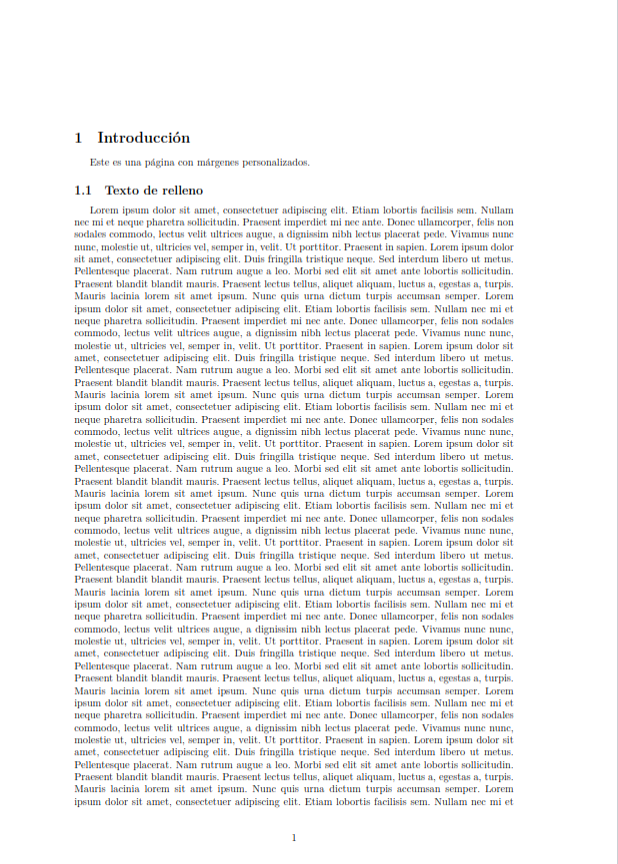
\includegraphics{./img/diseño-pagina/pagina-margenes-personalizados.png}
\end{tcolorbox}

\hypertarget{encabezados-y-pies-de-puxe1gina}{%
\section{Encabezados y pies de
página}\label{encabezados-y-pies-de-puxe1gina}}

\LaTeX incluye encabezados y pies de página automáticos dependiendo
del tipo de documento. Para las clases \texttt{article} y
\texttt{report} no hay encabezado y el pie es el número de página,
mientras que para la clase \texttt{book} el encabezado incluye la página
y la sección a la que corresponde la página. No obstante, el usuario
puede definir sus propios encabezados y pies mediante el paquete
\texttt{fancyhdr}.

Una vez cargado este paquete y antes de definir el texto del encabezado
y del pie, hay que cambiar el estilo de página (\texttt{plain} por
defecto) a \texttt{fancy}, y para ello se utiliza el comando
\texttt{\textbackslash{}pagestyle\{fancy\}} que indica al compilador que
se van a usar un encabezado y pie personalizados.

A continuación hay definir el texto del encabezado y del pie. El paquete
\texttt{fancyhdr} divide tanto el encabezado como el pie de página en
tres areas (izquierda, centro y derecha) e incorpora comandos para
escribir en cada una de ellas. El texto del área de la izquierda siempre
se justifica a la izquierda, el del área del centro se justifica
centrado y el del área derecha justificado a la derecha. Por otro lado,
para documentos a doble cara, se distingue también entre encabezados y
pies de páginas pares e impares.

Para definir el encabezado y el pie de página se utilizan los comandos

-\texttt{\textbackslash{}fancyhead{[}opcion{]}\{texo\}} añade el
\texttt{texto} al encabezado de página en el area que se indique en el
argumento opcional \texttt{opcion}, que puede ser \texttt{L} (área de la
izquierda), \texttt{C} (área del centro) o \texttt{R} (área de la
derecha), aunque para documentos a doble cara también se puede
especificar el encabezado para páginas pares añadiendo una \texttt{E} o
impares añadiendo una \texttt{O}.

-\texttt{\textbackslash{}fancyfoot{[}opcion{]}\{texo\}} añade el
\texttt{texto} al pie en el area que se indique en el argumento opcional
\texttt{opcion}.

\begin{tcolorbox}[enhanced jigsaw, arc=.35mm, toprule=.15mm, opacitybacktitle=0.6, colback=white, coltitle=black, colbacktitle=quarto-callout-warning-color!10!white, breakable, colframe=quarto-callout-warning-color-frame, left=2mm, opacityback=0, bottomtitle=1mm, toptitle=1mm, titlerule=0mm, title=\textcolor{quarto-callout-warning-color}{\faExclamationTriangle}\hspace{0.5em}{Advertencia}, bottomrule=.15mm, leftrule=.75mm, rightrule=.15mm]
El paquete \texttt{fancyhdr} no elimina los encabezados por defecto de
cada tipo de documento, por lo que si se van a definir encabezados o
pies personalizados, conviene utilizar los comandos
\texttt{\textbackslash{}fancyhead\{\}} y
\texttt{\textbackslash{}fancyfoot\{\}} para eliminar el encabezado y pie
por defecto antes de definir los propios.
\end{tcolorbox}

\textbf{Ejemplo}

\begin{Shaded}
\begin{Highlighting}[]
\CommentTok{\% PREÁMBULO}
\BuiltInTok{\textbackslash{}usepackage}\NormalTok{\{}\ExtensionTok{blindtext}\NormalTok{\}}
\BuiltInTok{\textbackslash{}usepackage}\NormalTok{\{}\ExtensionTok{fancyhdr}\NormalTok{\}}
\FunctionTok{\textbackslash{}pagestyle}\NormalTok{\{fancy\}}
\FunctionTok{\textbackslash{}fancyhead}\NormalTok{\{\} }\CommentTok{\% Borra el encabezado por defecto}
\FunctionTok{\textbackslash{}fancyhead}\NormalTok{[RO,LE]\{}\FunctionTok{\textbackslash{}textbf}\NormalTok{\{Mi encabezado\}\}}
\FunctionTok{\textbackslash{}fancyhead}\NormalTok{[C]\{Alfredo Sánchez\}}
\FunctionTok{\textbackslash{}fancyfoot}\NormalTok{\{\} }\CommentTok{\% Borra el pie por defecto}
\FunctionTok{\textbackslash{}fancyfoot}\NormalTok{[LE,RO]\{}\FunctionTok{\textbackslash{}thepage}\NormalTok{\}}
\FunctionTok{\textbackslash{}fancyfoot}\NormalTok{[LO,RE]\{}\FunctionTok{\textbackslash{}texttt}\NormalTok{\{http://aprendeconalf.es\}\}}

\CommentTok{\% CUERPO}
\KeywordTok{\textbackslash{}begin}\NormalTok{\{}\ExtensionTok{document}\NormalTok{\}}
\KeywordTok{\textbackslash{}section}\NormalTok{\{Introducción\}}
\NormalTok{Este es una página con encabezado y pie personalizado.}

\KeywordTok{\textbackslash{}subsection}\NormalTok{\{Texto de relleno\}}

\FunctionTok{\textbackslash{}blindtext}\NormalTok{[9]}
\KeywordTok{\textbackslash{}end}\NormalTok{\{}\ExtensionTok{document}\NormalTok{\}}
\end{Highlighting}
\end{Shaded}

\begin{tcolorbox}[enhanced jigsaw, arc=.35mm, toprule=.15mm, opacitybacktitle=0.6, colback=white, coltitle=black, colbacktitle=quarto-callout-note-color!10!white, breakable, colframe=quarto-callout-note-color-frame, left=2mm, opacityback=0, bottomtitle=1mm, toptitle=1mm, titlerule=0mm, title={Salida}, bottomrule=.15mm, leftrule=.75mm, rightrule=.15mm]
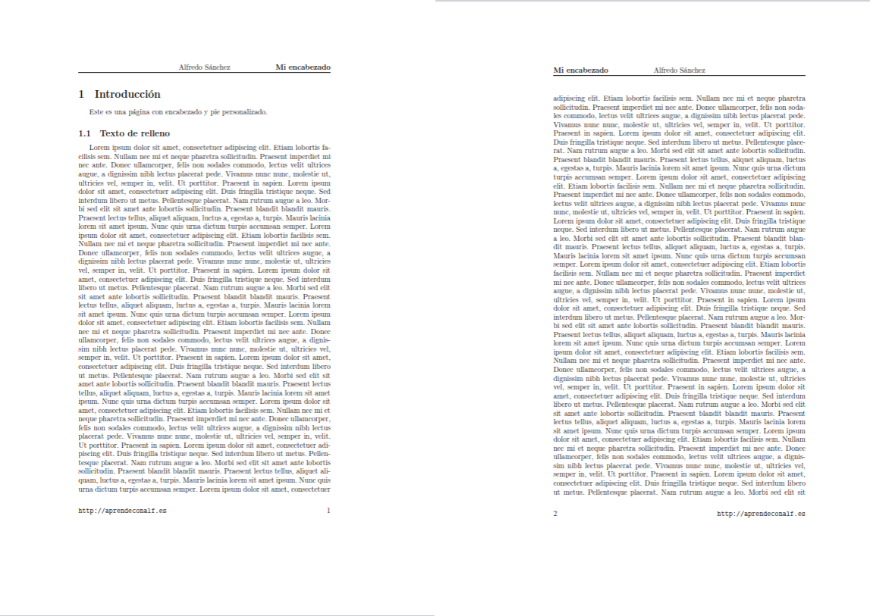
\includegraphics{./img/diseño-pagina/encabezado-pie.png}
\end{tcolorbox}

Como se puede observar, por defecto \texttt{fancyhdr} introduce una
línea horizontal para separar el encabezado. Es posible modificar el
grosor de la línea redefiniendo los comandos
\texttt{\textbackslash{}headrulewith} y
\texttt{\textbackslash{}footrulewith}. Por ejemplo, si no queremos que
aparezca la línea se escribiría
\texttt{\textbackslash{}renewcommand\{\textbackslash{}headrulewidth\}\{0pt\}}.

Finalmente, el espacio entre el encabezado y el cuerpo del texto también
se controla con el paquete \texttt{geometry} con la opción
\texttt{headsep=x}. Del mismo modo, la separación entre el pie y el
cuerpo se controla con la opción \texttt{footskip=x}.

\textbf{Ejemplo}

\begin{Shaded}
\begin{Highlighting}[]
\CommentTok{\% PREÁMBULO}
\BuiltInTok{\textbackslash{}usepackage}\NormalTok{\{}\ExtensionTok{blindtext}\NormalTok{\}}
\BuiltInTok{\textbackslash{}usepackage}\NormalTok{[top= 4cm, headsep=2cm]\{}\ExtensionTok{geometry}\NormalTok{\}}
\BuiltInTok{\textbackslash{}usepackage}\NormalTok{\{}\ExtensionTok{fancyhdr}\NormalTok{\}}
\FunctionTok{\textbackslash{}pagestyle}\NormalTok{\{fancy\}}
\FunctionTok{\textbackslash{}fancyhead}\NormalTok{\{\} }\CommentTok{\% Borra el encabezado por defecto}
\FunctionTok{\textbackslash{}fancyhead}\NormalTok{[R]\{}\FunctionTok{\textbackslash{}textbf}\NormalTok{\{Mi encabezado\}\}}
\FunctionTok{\textbackslash{}fancyhead}\NormalTok{[C]\{Alfredo Sánchez\}}
\FunctionTok{\textbackslash{}fancyfoot}\NormalTok{\{\} }\CommentTok{\% Borra el pie por defecto}
\FunctionTok{\textbackslash{}fancyfoot}\NormalTok{[R]\{}\FunctionTok{\textbackslash{}thepage}\NormalTok{\}}
\FunctionTok{\textbackslash{}fancyfoot}\NormalTok{[L]\{}\FunctionTok{\textbackslash{}texttt}\NormalTok{\{http://aprendeconalf.es\}\}}
\FunctionTok{\textbackslash{}renewcommand}\NormalTok{\{}\ExtensionTok{\textbackslash{}headrulewidth}\NormalTok{\}\{0pt\}}

\CommentTok{\% CUERPO}
\KeywordTok{\textbackslash{}begin}\NormalTok{\{}\ExtensionTok{document}\NormalTok{\}}
\KeywordTok{\textbackslash{}section}\NormalTok{\{Introducción\}}
\NormalTok{Este es una página con encabezado y pie personalizado.}

\KeywordTok{\textbackslash{}subsection}\NormalTok{\{Texto de relleno\}}

\FunctionTok{\textbackslash{}blindtext}\NormalTok{[9]}
\KeywordTok{\textbackslash{}end}\NormalTok{\{}\ExtensionTok{document}\NormalTok{\}}
\end{Highlighting}
\end{Shaded}

\begin{tcolorbox}[enhanced jigsaw, arc=.35mm, toprule=.15mm, opacitybacktitle=0.6, colback=white, coltitle=black, colbacktitle=quarto-callout-note-color!10!white, breakable, colframe=quarto-callout-note-color-frame, left=2mm, opacityback=0, bottomtitle=1mm, toptitle=1mm, titlerule=0mm, title={Salida}, bottomrule=.15mm, leftrule=.75mm, rightrule=.15mm]
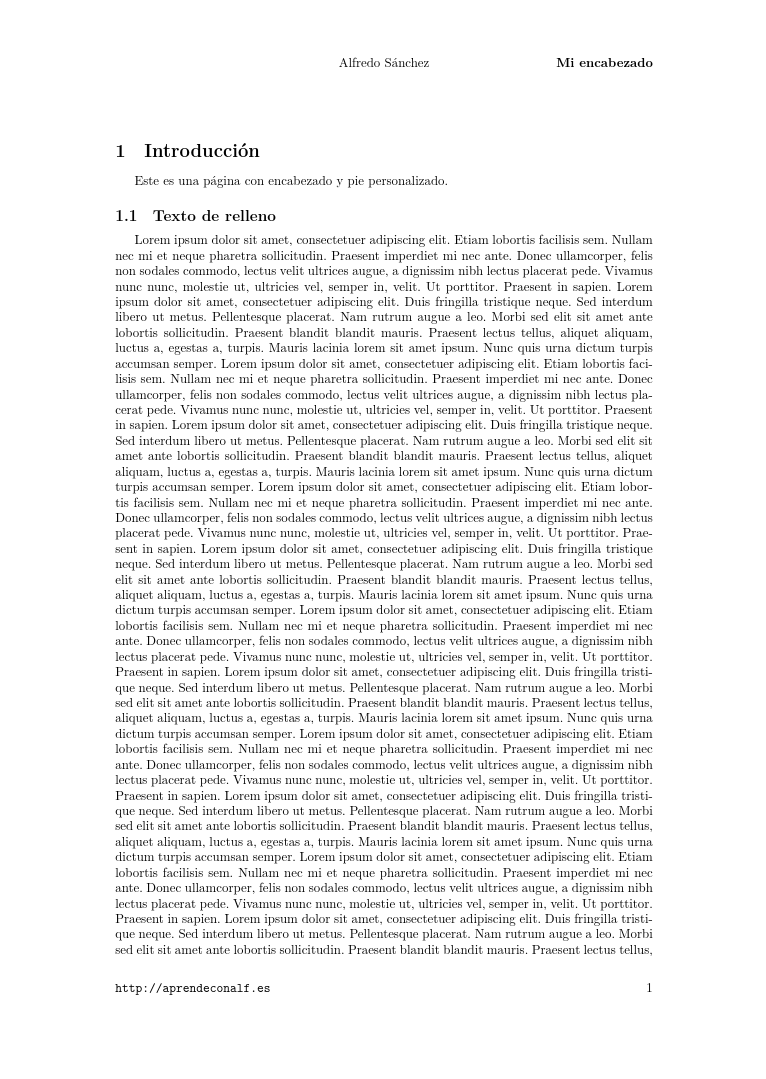
\includegraphics{./img/diseño-pagina/encabezado-pie-2.png}
\end{tcolorbox}

\bookmarksetup{startatroot}

\hypertarget{bibliografuxeda-y-recursos}{%
\chapter*{Bibliografía y recursos}\label{bibliografuxeda-y-recursos}}
\addcontentsline{toc}{chapter}{Bibliografía y recursos}

\hypertarget{libros}{%
\section*{Libros}\label{libros}}
\addcontentsline{toc}{section}{Libros}

\begin{itemize}
\tightlist
\item
  Cascales, B. y otros (2003). \emph{El libro de Latex}. Pearson
  Educación.
\item
  Cascales, B. y otros (2000). \emph{LaTeX: una imprenta en sus manos}.
  Aula Documental de Investigación.
\item
  Lamport, Leslie (1994). \emph{LaTeX: A Document Preparation System},
  2nd Edition. 2nd ed.~Addison-Wesley Professional. .
\item
  Mittelbach, F. et al.~(2004). \emph{LaTeX Companion, The, 2nd
  Edition}. 2nd ed.~Addison-Wesley Professional.
\item
  Oetiker, T et al (2021).
  \href{https://tobi.oetiker.ch/lshort/lshort.pdf}{\emph{The not so
  short introduction to LaTeX 2e}}
\end{itemize}

\hypertarget{sitios-web}{%
\section*{Sitios Web}\label{sitios-web}}
\addcontentsline{toc}{section}{Sitios Web}

\begin{itemize}
\tightlist
\item
  \href{https://www.latex-project.org/}{The \LaTeX project}. Sito
  web principal del proyecto \LaTeX con multitud de materiales para
  aprender y noticias sobre el desarrollo de nuevas versiones.
\item
  \href{https://ctan.org/}{Comprehensive \TeX Archive Network}.
  Principal repositorios de paquetes para \TeX y \LaTeX.
\item
  \href{www.cervantex.es/}{CervanTeX}. Grupos de usuarios de TeX
  hispanoablantes.
\item
  \href{https://project-awesome.org/egeerardyn/awesome-LaTeX}{Awesome
  LaTeX}. Sitio web con multitud de recursos curados para escribir
  documentos con \LaTeX.
\item
  \href{chulatex.pdf}{Chuleta de \LaTeX}. Resumen de los principales
  comandos y entornos de \LaTeX.
\end{itemize}



\end{document}
